\chapter[Dérivation des fonctions de la variable réelle]{Dérivation des fonctions à valeurs réelles de la variable réelle} 
\minitoc
\minilof
\minilot
Dans tout le chapitre $I$ désigne un intevalle réel non vide et non réduit à un point.
\section{Dérivation en un point}
\subsection{Dérivée en un point}
\subsubsection{Définition}
\begin{defdef}
  Soient $f \in \R^I$ et $a \in I$. On dit que $f$ est dérivable en $a$ si et seulement si $\lim\limits_{x \to a} \dfrac{f(x)-f(a)}{x-a}$ existe dans $\R$. On note $f'(a)$ cette limite finie si elle existe. Elle est appelée la dérivée de $f$ en $a$.
\end{defdef}
C'est équivalent à ce que $h \longrightarrow \frac{f(a+h)-f(a)}{h}$ admet une limite finie en zéro. Lorsqu'il existe $f'(a)$ est aussi noté $\derived{f}{x}(a)$. Avec les quantificateurs, si $f$ est dérivable en $a$, $f'(a)$ vérifie
\begin{equation}
  \forall \epsilon >0 \ \exists \eta > 0 \ \forall x \in I\setminus\{a\} \quad \abs{x-a} \leq \eta \implies \abs{\frac{f(x)-f(a)}{x-a} - f'(a)} \leq \epsilon.
\end{equation}

\subsubsection{Interprétation graphique}

Soient $f \in \R^I$ et $a \in I$. On suppose que $f$ est dérivable en $a$. On définit deux fonctions
\begin{align}
  &\fonction{\varphi}{I}{\R}{x}{\begin{cases}\frac{f(x)-f(a)}{x-a} & x \neq a, \\ f'(a) & x=a\end{cases}} \\ 
  &\fonction{\epsilon}{I}{\R}{x}{\begin{cases}\frac{f(x)-f(a)}{x-a} -f'(a)& x \neq a \\ 0 & x=a\end{cases}}
\end{align}
%
\begin{prop}
  Les fonctions $\varphi$ et $\epsilon$ sont toutes les deux continues en $a$. De plus
  \begin{equation}
    \forall x \in I \quad \varphi(x) = \epsilon(x) +f'(a).
  \end{equation}
  La fonction $f$ admet le développement limité à l'ordre un suivant
  \begin{equation}
    \forall x \in I \quad f(x) = f(a) + f'(a)(x-a) + \epsilon(x)(x-a),
  \end{equation}
  avec $\lim\limits_{a} \epsilon=0$. Soit $h$ la partie régulière du $DL_1(a)$ de $f$, c'est une fonction affine appelée fonction affine tangente. La droite d'équation $y=f(a)+f'(a)(x-a)$ est tangente à la courbe représentative de $f$ au point $A(a,f(a))$.
% Par exemple on peut donner la tangente de la fonction $f : x \longrightarrow \frac{1}{x} - \frac{x^2-2}{x-10}$ au point d'abcisse $\sqrt{2}$ sur la figure~\ref{fig:derivee}. 
% \begin{figure}
%   \centering
%   \includegraphics[angle=-90,scale=1,width=0.6\textwidth]{./derivee.ps}
%   \caption{Dérivée en un point d'une fonction}
%   \label{fig:derivee}
% \end{figure}
% La tangente en $A$ est la position limite des cordes lorsque $M(x,f(x))$ tend vers $A$.
\end{prop}
%
Lorsque $\frac{f(x)-f(a)}{x-a}$ tend vers $\pm\infty$ alors la tangente est verticale. La fonction n'est dans ce cas pas dérivable en $a$.

\subsubsection{Interprétation cinématique}
Si on suppose que $f(t)$ représente la position d'un point mobile $M(t)$ à l'innstant $t$~:
\begin{itemize}
\item $\frac{f(t)-f(a)}{t-a}$ est la vitesse moyenne du point $M$ entre les instants $a$ et $t$;
\item $f'(a)$ est la vitesse instantannée à l'instant $a$.
\end{itemize}

\subsection{Dérivée à droite, dérivée à gauche}

\subsubsection{Définition}
Soit $f \in \R^I$, $a \in I$ et on suppose que $I \cap \intervalleoo{a}{+\infty}$ est non vide.
\begin{defdef}
  On dit que $f$ est dérivable à droite en $a$ lorsque la restriction de $f$ à $I \cap \intervalleoo{a}{+\infty}$ est dérivable en $a$. C'est équivalent à
  \begin{enumerate}
  \item la fonction $\fonction{h_1}{I\setminus\{a\}}{\R}{x}{\frac{f(x)-f(a)}{x-a}}$ admet une limite finie à droite en $a$;
  \item la fonction $\fonction{h_2}{I \cap \intervalleoo{a}{+\infty}}{\R}{x}{\frac{f(x)-f(a)}{x-a}}$ admet une limite finie en $a$.
  \end{enumerate}
  Sous réserve d'existence de cette limite, on note $f'_d(a) = \lim\limits_{x \to a^+}\frac{f(x)-f(a)}{x-a}$. On définit de manière analogue la dérivée à gauche en $f$. On note $f'_g(a) = \lim\limits_{x \to a^-}\frac{f(x)-f(a)}{x-a}$ lorsque la limite existe et est finie..
\end{defdef}

\subsubsection{Propriétés}

Soit $f \in \R^I$ et $a \in I$.
\begin{prop}
  Si $f$ est dérivable en $a$ et si $I\cap \intervalleoo{a}{+\infty}$ est non vide, alors $f$ est dérivable à droite en $a$ et $f'_d(a)=f'(a)$. La réciproque est fausse.
\end{prop}
\begin{prop}
  Si $f$ est dérivable en $a$ et si $I\cap \intervalleoo{-\infty}{a}$ est non vide, alors $f$ est dérivable à gauche en $a$ et $f'_g(a)=f'(a)$. La réciproque est fausse.
\end{prop}
\begin{prop}
  Si $a$ appartient à l'intérieur de $I$ (c'est-à-dire si $I\cap \intervalleoo{a}{+\infty}$ et $\intervalleoo{-\infty}{a}$ sont non vides) alors $f$ est dérivable en $a$ si et seulement si $f$ est dérivable à gauche et à droite en $a$ et si $f'_g(a) = f'_d(a)$ et auquel cas $f'_g(a)=f'_d(a)=f'(a)$.
\end{prop}
\begin{proof}
  Les deux premières propositions découlent de la définition. La troisième découle des deux premières.
\end{proof}

\subsubsection{Dérivabilité et continuité}

\begin{prop}
  Soit $f \in \R^I$, $a \in I$. Si $f$ est dérivable en $a$ alors elle est continue en $a$. La réciproque est fausse.
\end{prop}
\begin{proof}
  On avait vu que si $f$ est dérivable alors elle admet le développement limité à l'ordre 1 suivant
  \begin{equation}
    \forall x \in I \quad f(x)=f(a)+f'(a)(x-a)+(x-a)\epsilon(x),
  \end{equation}
  avec $\epsilon$ de limite nulle en $a$ (donc continue en $a$). La fonction $x \longrightarrow x-a$ est continue alors par produit $x \longmapsto (x-a)\epsilon(x)$ est continue en $a$. La fonction affine $x \longrightarrow f(a)+f'(a)(x-a)$ est continue en $a$. Ainsi par somme $f$ est continue en $a$.
\end{proof}
La réciproque est fausse, on peut avoir des fonctions continues qui ne sont pas dérivables, comme par exemple la valeur absolue en zéro. On peut avoir des fonctions continue en tout point mais dérivable nulle part, comme par exemple la trajectoire du mouvement brownien.

\subsection{Extremums locaux et dérivées}

\subsubsection{Définitions}

Soit $f \in \R^I$, $a \in I$, on dit que
\begin{enumerate}
\item $f$ admet un maximum global en $a$ si $\forall x \in I \quad f(x) \leq f(a)$;
\item $f$ admet un minimum global en $a$ si $\forall x \in I \quad f(x) \geq f(a)$;
\item $f$ admet un extremum global en $a$ si elle admet un maximum ou un minimum global en $a$;
\item $f$ admet un maximum local en $a$ si $\exists h > 0 \forall x \in I \cap \intervalleoo{a-h}{a+h}  \quad f(x) \leq f(a)$;
\item $f$ admet un minimum local en $a$ si $\exists h > 0 \forall x \in I \cap \intervalleoo{a-h}{a+h} \quad f(x) \geq f(a)$;
\item $f$ admet un extremum local en $a$ si elle admet un maximum ou un minimum local en $a$;
\item On définit les notions d'extremum stricts de la même manière en remplaçant $\leq$ resp.\ $\geq$ par $<$ resp.\ $>$.
\end{enumerate}

\subsubsection{Liens avec les dérivées}

\begin{theo}
  Soient $f \in \R^I$ et $a \in I$ qui n'est pas une borne de $I$. On suppose que $f$ est dérivable en $a$ et que $f$ admet un extremum local en $a$. Alors $f'(a)=0$.
\end{theo}
\begin{proof}
  On suppose par exemple que $f$ admet un maximum local en $a$. Le réel $a$ est dans l'intérieur de $I$ donc il existe $h_1>0$ tel que $\intervalleff{a-h_1}{a+h_1} \subset I$. La fonction $f$ admet un maximum local en $a$ donc il existe $h_2>0$ tel que pour tout $x \in I \cap \intervalleff{a-h_2}{a+h_2}$, $f(x) \leq f(a)$. Soit $h_0=\min(h_1,h_2)$ alors $\intervalleff{a-h_0}{a+h_0} \cap A = \intervalleff{a-h_0}{a+h_0}$. Soit $x \in \intervalleff{a-h_0}{a+h_0}$,
  \begin{itemize}
  \item Si $x > a$ alors $\frac{f(x)-f(a)}{x-a} \leq 0$ et donc par passage à la limite $f'_d(a) \leq 0$;
  \item Si $x < a$ alors $\frac{f(x)-f(a)}{x-a} \geq 0$ et donc par passage à la limite $f'_g(a) \geq 0$.
  \end{itemize}
  Or on sait que $f$ est dérivable en $a$, donc $0 \leq f'_d(a)=f'_g(a) \leq 0$. Donc $f'(a)=0$.
\end{proof}

La réciproque est fausse, un contre-exemple suffisant est la fonction cube en zéro. Sa dérivée est nulle et pourtant elle n'admet pas d'extremum. En fait c'est un point d'inflexion. Cependant une fonction peut admettre un extremum en un point où elle n'est pas dérivable. En effet, la fonction valeur absolue admet zéro comme minimum global en zéro alors qu'elle n'est pas dérivable en zéro.

\subsection{Dérivabilité en un point et existence d'un développement limité à l'ordre un}
On a déja dit que si $f$ est dérivable en $a$, alors elle admet un $DL_1(a)$. De manière réciproque on peut énoncer la proposition suivante
\begin{prop}
  Soit $f \in \R^I$, $a \in I$. On suppose que $f$ admet le $DL_1(a)$ suivant
  \begin{equation}
    f(x)=\alpha_0 +\alpha_1(x-a) +(x-a) \epsilon(x) \quad \lim_a \epsilon =0,
  \end{equation}
  alors $f$ est dérivable en $a$ et $\alpha_0=f(a)$ et $f'(a)=\alpha_1$.
\end{prop}
\begin{proof}
  On a déjà vu que $\alpha_0=f(a)$, par troncature. D'autre part
  \begin{equation}
    \forall x \in I\setminus\{a\} \quad \frac{f(x)-f(a)}{x-a} = \alpha_1 +\epsilon(x).
  \end{equation}
  En passant à la limite, puisque $\epsilon$ tend vers zéro en $a$, on a bien $f'(a)=\alpha_1$.
\end{proof}
Cependant, la propriété n'est pas généralisable pour un $DLn(a)$ où $n \geq 2$.

\subsubsection{Interprétation graphique du $DL_1(a)$}

Si $f$ admet le $DL_1(a)$ $f(x)=\alpha_0 +\alpha_1(x-a) +\petitof{a}{(x-a)}$ avec $x \longrightarrow \alpha_0 +\alpha_1(x-a)$ la fonction affine tangente. On suppose que $f$ admet un $DL_n(a)$ avec $n \geq 2$,
\begin{equation}
  f(x) = \sum_{k=0}^n \alpha_k (x-a)^k +\petitof{a}{(x-a)^n},
\end{equation}
tel qu'il existe $k \in \intervalleentier{2}{n}$ et $\alpha_k \neq 0$. Si $p=\min\enstq{k \in \intervalleentier{2}{n}}{\alpha_k \neq 0}$ alors
\begin{equation}
  f(x) - \alpha_0 - \alpha_1(x-a) \sim_a \alpha_p (x-a)^p.
\end{equation}
On peut donc étudier la position relative de la courbe représentative de $f$ par rapport à sa tangente en $a$ en fonction du signe du réel $\alpha_p$ et de la parité du naturel $p$.

\subsection{Fonction dérivée. Opérations algébriques}

\subsubsection{Fonction dérivée}

Soient $I$ un intervalle contenant au moins deux points et un réel $a \in I$. On note $\derivpt{a}{I}{\R}$ l'ensemble des fonctions de I vers $\R$ qui sont dérivables en $a$. On dit que $f$ est dérivable sur $I$ si elle est continue en tout point de $I$. On note $\deriv{I}{\R}$ l'ensemble des fonctions de I dans $\R$ dérivables sur $I$. On a $\deriv{I}{\R}=\bigcap\limits_{a \in I} \derivpt{a}{I}{\R}$.

Lorsque $f$ est dérivable sur $I$, on peut définir l'application
\begin{equation}
  \fonction{f'}{I}{\R}{a}{f'(a)}.
\end{equation}
Cette application est appelée la dérivée de $f$. On note $\classe{1}(I,\R)$ l'ensemble des fonctions de $\deriv{I}{\R}$ telle que la fonction dérivée est continue sur $I$.
\begin{equation}
  \classe{1}(I,\R) \subsetneq \deriv{I}{\R} \subsetneq \cont{I}{\R}.
\end{equation}
Les inclusions sont strictes, puisqu'une fonction peut être continue sans être dérivable et dérivable sans que sa dérivée soit continue. On dispose des applications suivantes
\begin{gather}
  \fonction{\varphi}{\derivpt{a}{I}{\R}}{\R}{f}{f'(a)}; \\ 
  \fonction{\psi}{\deriv{I}{\R}}{\R^I}{f}{f'}; \\ 
  \fonction{\zeta}{\classe{1}(I,\R)}{\cont{I}{\R}}{f}{f'}.
\end{gather}

\subsubsection{Somme}

\begin{theo}
  L'ensemble $\derivpt{a}{I}{\R}$ est un sous-espace vectoriel de $\R^I$. Autrement dit l'application $\varphi$ est linéaire.
\end{theo}
\begin{proof}
  Soient $f$ et $g$ deux applications dérivables sur $I$, un réel $\lambda$. Alors pour tout $x \in I\setminus\{a\}$
  \begin{equation}
    \frac{(\lambda f +g)(x)-(\lambda f +g)(a)}{x-a} = \lambda \frac{f(x)-f(a)}{x-a} + \frac{g(x)-g(a)}{x-a}.
  \end{equation}
  En passant à la limite en $a$, on a
  \begin{equation}
    (\lambda f+g)'(a)=\lambda f'(a)+g'(a).
  \end{equation}
\end{proof}
\begin{corth}
  L'ensemble $\deriv{I}{\R}$ est un sous-espace vectoriel de $\R^I$. Autrement dit l'application $\psi$ est linéaire.
\end{corth}
\begin{corth}
  L'ensemble $\classe{1}(I,\R)$ est un sous-espace vectoriel de $\R^I$. Autrement dit l'application $\zeta$ est linéaire.
\end{corth}

\subsubsection{Produit}

\begin{theo}
  Soient $f$ et $g$ deux applications de $\derivpt{a}{I}{\R}$ alors $fg \in \derivpt{a}{I}{\R}$ et
  \begin{equation}
    (fg)'(a)=f'(a)g(a)+f(a)g'(a)
  \end{equation}
\end{theo}
\begin{proof}
  Soit un réel $x \in I \setminus \{a\}$ alors
  \begin{equation}
    \frac{(fg)(x)-(fg)(a)}{x-a} = \frac{f(x)-f(a)}{x-a}g(x) + f(a)\frac{g(x)-g(a)}{x-a}.
  \end{equation}
  Donc, puisque $f$ et $g$ sont dérivable en $a$, en passant à la limite en $a$ on a bien
  \begin{equation}
    (fg)'(a)=f'(a)g(a)+f(a)g'(a).
  \end{equation}
\end{proof}
\begin{corth}
  Soient $f$ et $g$ deux applications de $\deriv{I}{\R}$n alors $fg \in \deriv{I}{\R}$ et
  \begin{equation}
    (fg)'=f'g+fg'.
  \end{equation}
\end{corth}
\begin{corth}
  Soient $f$ et $g$ deux applications de $\classe{1}(I,\R)$n alors $fg \in \classe{1}(I,\R)$ et
  \begin{equation}
    (fg)'=f'g+fg'.
  \end{equation}
\end{corth}
En particulier, si $f$ est dans $\deriv{I}{\R}$ alors pour tout naturel $n$ non nul $f^n \in \deriv{I}{\R}$ et $\left(f^n\right)'=nf' f^{n-1}$ (preuve par récurrence facile à vérifier).

\subsubsection{Inverse et quotient}

\begin{theo}
  Soit une fonction $g \in \derivpt{a}{I}{\R}$ qui ne s'annule pas en $a$. Alors il existe un voisinage de $a$ dans le quel $g$ ne s'annule pas. Soit $U$ un tel voisinage. Alors $\frac{1}{g}$ est définie et dérivable sur $U$ telle que
  \begin{equation}
    \left(\frac{1}{g}\right)'(a) = \frac{-g'(a)}{g(a)^2}.
  \end{equation}
  Pour toute fonction $f$ dérivable sur I, alors $\frac{f}{g}$ est dérivable sur $U$ et
  \begin{equation}
    \left(\frac{f}{g}\right)'(a) = \frac{f'(a)g(a)-f(a)g'(a)}{g(a)^2}.
  \end{equation}
\end{theo}
\begin{proof}
  La fonction $g$ est dérivable en $a$, donc elle est continue en $a$ et $g(a) \neq 0$. Il existe donc un voisinage $U$ de $a$ sur lequel $g$ ne s'annule pas.
  \begin{equation}
    \forall x \in U\setminus\{a\} \quad \frac{\left(\frac{1}{g}\right)(x)-\left(\frac{1}{g}\right)(a)}{x-a} = \frac{-1}{g(x)g(a)} \frac{g(x)-g(a)}{x-a}.
  \end{equation}
  En passant à la limite en $a$, puisque $g$ est dérivable en $a$, alors par produit de limite on a bien
  \begin{equation}
    \left(\frac{f}{g}\right)'(a) = \frac{f'(a)g(a)-f(a)g'(a)}{g(a)^2}.
  \end{equation}
  Pour le quotient, on applique le premier point et le résultat sur les produits.
\end{proof}
%
\begin{corth}
  Soient $f$ et $g$ dans $\deriv{I}{\R}$ telles que $g$ ne s'annule pas sur $I$, alors $\frac{f}{g} \in \deriv{I}{\R}$ et
  \begin{equation}
    \left(\frac{f}{g}\right)' = \frac{f'g-fg'}{g^2}.
  \end{equation}
\end{corth}
\begin{corth}
  Soient $f$ et $g$ dans $\classe{1}(I,\R)$ telles que $g$ ne s'annule pas sur $I$, alors $\frac{f}{g} \in \classe{1}(I,\R)$ et
  \begin{equation}
    \left(\frac{f}{g}\right)' = \frac{f'g-fg'}{g^2}.
  \end{equation}
\end{corth}
On montre par récurrence que si $f$ est dérivable et ne s'annule pas sur I alors pour tout $n \in \Z\setminus \N$, $f^n$ est dérivable sur $I$.

\subsubsection{Dérivée logarithmique}

\begin{defdef}
  Soit $f \in \derivpt{a}{I}{\R}$ qui ne s'annule pas en $a$. On appelle dérivée logarithmique de $f$ en $a$ le réel $\frac{f'(a)}{f(a)}$.
\end{defdef}
\begin{theo}
  Soient deux fonction $f$ et $g$ de $\derivpt{a}{I}{\R}$ qui ne s'annulent pas en $a$. Alors
  \begin{gather}
    \frac{(fg)'(a)}{(fg)(a)}=\frac{f'(a)}{f(a)}+\frac{g'(a)}{g(a)}; \\
    \forall \lambda \in \R^{*} \quad \frac{(\lambda f)'(a)}{(\lambda f)(a)}=\frac{f'(a)}{f(a)}; \\
    \frac{(f/g)'(a)}{(f/g)(a)}=\frac{f'(a)}{f(a)}-\frac{g'(a)}{g(a)}; \\
    \forall \alpha \in \Z \quad \frac{(f^\alpha)'(a)}{(f^\alpha)(a)}= \alpha \frac{f'(a)}{f(a)}.
  \end{gather}
\end{theo}
Ce théorème est parfois utile pour calculer les dérivées de produits ou de quotient.

\subsection{Composition de fonctions dérivables}

\begin{theo}
  Soient $I$ et $J$ deux intervalles de $\R$. Soit $f \in \R^I$, $g \in \R^J$ avec $f(I) \subset J$. Si $f$ est dérivable en $a$ et $g$ est dérivable en $f(a)$ alors $f \circ g$ est dérivabele en $a$ et
  \begin{equation}
    (g \circ f)'(a)=f'(a) (g' \circ f)(a).
  \end{equation}
\end{theo}
\begin{proof}
  On sait que
  \begin{equation}
    \forall x \in I\setminus\{a\} \quad \frac{g \circ f(x) -g \circ f(a)}{x-a} = \frac{g \circ f(x) -g \circ f(a)}{f(x)-f(a)} \frac{f(x)-f(a)}{x-a}.
  \end{equation}
  Puisque $f$ est dérivable en $a$, on a bien $\lim\limits_{x \to a} \frac{f(x)-f(a)}{x-a} = f'(a)$ et elle est continue en $a$, donc $\lim\limits_{x \to a} f(x)=f(a)$. La fonction $g$ est dérivable en $f(a)$ donc $\lim\limits_{y \to f(a)} \frac{g(y)-g(f(a))}{y-f(a)} = g'(f(a))$. Par composition de limites, on en déduit que $\lim\limits_{x \to a} \frac{g(f(x))-g(f(a))}{f(x)-f(a)} = g'(f(a))$. Donc par produit, $\lim\limits_{x \to a} \frac{g \circ f(x) -g \circ f(a)}{x-a} = g'(f(a)) f'(a)$.
\end{proof}
\begin{corth}
  Soient deux fonctions $f \in \deriv{I}{\R}$ et $g \in \Dr(J)$ telles que $f(I) \subset J$, alors $g \circ f \in \deriv{I}{\R}$ et $(g\circ f)'=f' \cdot g' \circ f$.
\end{corth}
\begin{corth}
  Soient deux fonctions $f \in \classe{1}(I,\R)$ et $g \in \classe{1}(J)$ telles que $f(I) \subset J$, alors $g \circ f \in \classe{1}(I,\R)$.
\end{corth}

\emph{Exemples}

\begin{enumerate}
\item Si $f \in \deriv{I}{\R}$ (resp.\ $\classe{1}(I,\R)$) alors $\e^f \in \deriv{I}{\R}$ (resp.\ $\classe{1}(I,\R)$) et $(\e^f)'=f' \e^f$;
\item si $f \in \deriv{I}{\R}$ qui ne s'annule pas, alors $\ln \abs{f} \in \deriv{I}{\R}$ et $\left(\ln\abs{f} \right)'=\frac{f'}{f}$;
\item si $f \in \deriv{I}{\R}$ et $f(I) \subset \Rplusetoile$ et $\alpha \in \R$ alors $f^\alpha \in \deriv{I}{\R}$ et $(f^\alpha)'=\alpha f' f^{\alpha-1}$;
\item si $f \in \deriv{I}{\R}$ avec $f(I) \subset \Rplusetoile$ et $u \in \deriv{I}{\R}$ alors $f^u=\e^{u \ln f} \in \deriv{I}{\R}$ et $(f^u)'=\left(u'\ln f+u \frac{f'}{f}\right) f^u$.
\end{enumerate}

\subsection{Dérivation d'une fonction réciproque}

\begin{theo}
  Soit $I$ un intervalle réel et $a \in I$. Soit $f \in \cont{I}{\R}$ strictement monotone. Alors $f$ induit une bijection de $I$ sur $f(I)=J$ dont on note $f^{-1}$ l'application réciproque. Alors
  \begin{equation}
    f \in \Dr_{a}(I) \text{~et~} f'(a) \neq 0 \implies f^{-1} \in \Dr_{f(a)}(J) \text{~et~} (f^{-1})'(f(a))=\frac{1}{f'(a)}.
  \end{equation}
\end{theo}
\begin{proof}
  Soit $y \in J \setminus \{f(a)\}$, on note $x=f^{-1}(y)$. Alors
  \begin{equation}
    \frac{f^{-1}(y)-f^{-1}(f(a))}{y-f(a)}=\frac{x-a}{f(x)-f(a)} = \frac{1}{\varphi_{f,a}(x)}=\frac{1}{\varphi_{f,a}(f^{-1}(y))}.
  \end{equation}
  Comme $f^{-1}$ est continue, on a $\lim\limits_{y \to f(a)}f^{-1}(y) = a$ et comme $f$ est dérivable $\lim\limits_{x \to a} \varphi_{f,a}(x)=f'(a)$. Donc par composition de limite on a $\lim\limits_{y \to f(a)}\varphi_{f,a}(f^{-1}(y))=f'(a)$. Comme $f'(a)$ n'est pas nul on peut l'inverser et $f^{-1}$ est dérivable en $f(a)$, et~:
  \begin{equation}
    (f^{-1})'(f(a))=\frac{1}{f'(a)} = \lim\limits_{y \to f(a)} \frac{f^{-1}(y)-f^{-1}(f(a))}{y-f(a)} = \frac{1}{f'(a)}.
  \end{equation}
\end{proof}
\begin{corth}
  Soit $I$ un intervalle réel, $f \in \R^I$ strictement monotone, dérivable sur $I$ et $f'$ ne s'annule pas sur $I$. Alors $f$ induit une bijection de $I$ sur $J=f(I)$ et l'application réciproque $f^{-1}$ est dérivable sur $J$ et de plus
  \begin{equation}
    (f^{-1})'=\frac{1}{f' \circ f^{-1}}.
  \end{equation}
\end{corth}
\begin{corth}
  Sous les mêmes hypothèses, si on suppose que $f \in \classe{1}(I,\R)$ alors $f^{-1} \in \classe{1}(I,\R)$.
\end{corth}

Que se passe-t-il si $f'$ s'annule en $a$?

Comme $f$ est strictement monotone, la fonction $\varphi_{f,a}$ est à valeurs soit strictement positives soit strictement négatives. La limite en $f(a)$ de $\frac{1}{\varphi_{f,a}}$ est infinie. Alors $f^{-1}$ n'est pas dérivable en $f(a)$ mais la courbe représentative de $f^{-1}$ admet une tangente verticale en $(f(a),a)$. Comme par exemple la fonction argument cosinus hyperbolique en un.

\subsection{Dérivées successives}

\subsubsection{Définitions et notations}

Soit $I$ un intervalle réel et $f \in \R^I$. Si $f$ est dérivable en tout point $a$ de $I$, alors on dispose de l'application $f'$ qui associe le réel $a$ eu réel $f'(a)$. Si $f'$ est définie et continue sur $I$, alors on dit que $f$ est de classe $\classe{1}$ sur $I$.

Si $f'$ est définie sur $I$ et si $f'$ est dérivable en un point $a \in I$, le réel $(f')'(a)$ noté $f''(a)$ est la dérivée seconde de $f$ en $a$. Si $f'$ est définie et dérivable en tout point $a$ de $I$ on note sa dérivée l'application $f''$ ou encore $f^{(2)}$. Si $f''$ est continue sur $I$ on dit que $f$ est de classe $\classe{2}$.

On itére le processus. Supposons que $f^{(k-1)}$ est définie sur $I$. Si $f^{(k-1)}$ est dérivable en $a \in I$ on note $f^{(k)}(a)$ le nombre dérivé $(f^{(k-1)})'(a)$ et on dit que $f$ est $k$ fois dérivable en $a$. Si $f^{(k-1)}$ est définie et dérivable sur $I$ on note $f^{(k)} = (f^{(k-1)})'$ et on dit que $f$ est $k$ fois dérivable sur $I$.

Ne pas confondre $f^{(k)}$ qui est la dérivée $k$\ieme de $f$ avec la puissance $f^k$. Si $f^{(k)}$ est continue sur I, alors on dit que $f$ est de classe $\classe{k}$ sur $I$.

Finalement sous réserve d'existence, $f^{(0)}=f$ et pour tout naturel $n$, $f^{(n+1)}=(f^{(n)})'=(f')^{(n)}$. Soit un naturel $n$, alors
\begin{itemize}
\item $f$ est dite $\Dr^n$ lorsqu'elle est dérivable $n$ fois sur $I$. On note $\derivnfois{n}{I}{\R}$ l'ensemble des fonctions qui sont $\Dr^n$ sur I;
\item $f$ est dite $\classe{n}$ lorsqu'elle est dérivable $n$ fois sur $I$ et que $f^{(n)}$ est continue. On note $\classe{n}(I)$ l'ensemble des applications qui sont $\classe{n}$ sur I;
\item $f$ est dite $\classe{\infty}$ lorsque pour tout naturel $n$, $f$ est $\classe{n}$; on note
  \begin{equation}
    \classe{\infty}(I,\R)=\bigcap\limits_{n \in \N} \classe{n}(I,\R).
  \end{equation}
\end{itemize}
On a donc les inclusions suivantes~:
\begin{equation}
  \classe{\infty}(I,\R) \subsetneq \cdots \subsetneq \classe{{n+1}}(I,\R) \subsetneq \derivnfois{n+1}{I}{\R} \subsetneq \classe{n}(I,\R) \subsetneq \cdots \subsetneq \cont{I}{\R} \subsetneq \R^I.
\end{equation}
Les inclusions sont strictes.
\begin{prop}
  L'égalité suivante est vraie
  \begin{equation}
    \classe{\infty}(I,\R) = \bigcap\limits_{n \in \N} \derivnfois{n}{I}{\R}
  \end{equation}
\end{prop}
\begin{proof}
  Soit $n \in \N$ alors $\classe{n}(I,\R) \subset \derivnfois{n}{I}{\R}$. Donc $\classe{\infty}(I,\R) \subset \bigcap\limits_{n \in \N} \derivnfois{n}{I}{\R}$.

  Soit $f \in \bigcap\limits_{n \in \N} \derivnfois{n}{I}{\R}$, alors pour tout naturel $n$ $f \in \derivnfois{n+1}{I}{\R}$ alors $f \in \classe{n}(I,\R)$. Finalement $f \in \classe{\infty}(I,\R)$. On dira que $f$ est indéfiniment dérivable.
\end{proof}

\subsubsection{Opérations algébriques et théorème de Leibniz}

\begin{theo}
  Soient $n$ un naturel non nul, $\lambda$ un réel, $f$ et $g$ deux applications de $I$ dans $\R$.
  \begin{enumerate}
  \item Si $f$ et $g$ sont $n$ fois dérivables alors $\lambda f +g$ l'est aussi et $(\lambda f +g)^{(n)}=\lambda f^{(n)} + g^{(n)}$ et $fg$ est aussi $n$ fois dérivable telle que $(fg)^{(n)}=\sum_{k=0}^n \binom{n}{k} f^{(k)}g^{(n-k)}$;
  \item si $f$ et $g$ sont de classe $\classe{n}$ alors $\lambda f +g$ et $fg$ sont aussi de classe $\classe{n}$;
  \item si $f$ et $g$ sont de classe $\classe{\infty}$ alors $\lambda f +g$ et $fg$ sont aussi de classe $\classe{\infty}$.
  \end{enumerate}
\end{theo}
\begin{proof}
  La linéarité de $f \longmapsto f^{(n)}$ se démontre par réccurence à partir de la linéarité de $f \longmapsto f'$. C'est assez facile. Par contre le morceaux le plus difficile est la formule de Leibniz. Soit un naturel $n$, on définit la propriété $\P(n)$
  \begin{equation}
    \forall (f,g) \in \derivnfois{n}{I}{\R}^2 \quad fg \in \derivnfois{n}{I}{\R} \text{~et~} (fg)^{(n)}=\sum_{k=0}^n \binom{n}{k} f^{(k)}g^{(n-k)}.
  \end{equation}

Soit $n=1$, alors si $f$ et $g$ sont dérivables, alors on sait que $fg$ est dérivable d'après les propriétés et $(fg)'=f'g+g'f=\sum_{k=0}^1 \binom{1,k} f^{(k)}g^{(1-k)}$. Donc $\P(1)$ est vraie.

Supposons maintenant $\P(n)$ pour $n \neq 0$, montrons $\P(n+1)$. Soit $f$ et $g$ $n+1$ fois dérivables, alors elles le sont $n$ fois et par hypothèse de récurrence $(fg)^{(n)}=\sum_{k=0}^n \binom{n}{k} f^{(k)}g^{(n-k)}$. Pour tout $k \leq n$ $f^{(k)}$ et $g^{(n-k)}$ sont dérivables (puisque $f$ et $g$ le sont $n+1$ fois). Par produit est combinaisons linéaires de fonctions dérivables, la fonction $(fg)^{(n)}$ est dérivable. Autrement dit $fg$ est $n+1$ fois dérivable et
\begin{align}
  (fg)^{(n+1)}=\left((fg)^{(n)}\right)'&=\sum_{k=0}^n \binom{n}{k} [f^{(k)}g^{(n-k)}]' \\
  &=\sum_{k=0}^n \binom{n}{k} [f^{(k+1)}g^{(n-k)}+f^{(k)}g^{(n-k+1)}]\\
  &=\sum_{k=0}^n \binom{n}{k} f^{(k+1)}g^{(n-k)} + \sum_{k=0}^n \binom{n,k} f^{(k)}g^{(n-k+1)}.
\end{align}
On change de variable $j=k+1$ dans la première somme et on obtient
\begin{align}
  (fg)^{(n+1)}&=\sum_{j=1}^{n+1} \binom{n}{j-1} f^{(j)}g^{(n+1-j)} + \sum_{k=0}^n \binom{n}{k} f^{(k)}g^{(n-k+1)}\\
  &= \binom{n}{n} f^{(n+1)}g^{(0)} + \sum_{j=1}^n \left[\binom{n}{j-1}+\binom{n}{j}\right]f^{(j)}g^{(n+1-j)} + \binom{n}{0} f^{(0)}g^{(n+1)}\\
  &= \sum_{j=0}^{n+1} \binom{n+1}{j}f^{(j)}g^{(n+1-j)}.
\end{align}
Alors $\P(n+1)$ est vraie. Par théorème de récurrence, $\P(n)$ est vraie pour tout naturel $n$ non nul.
\end{proof}

\begin{theo}
  Soient deux applications $f$ et $g$ de $I$ dans $\R$ telles que $g$ ne s'annulent pas sur $I$. Soit un naturel $n$ non nul.
  \begin{enumerate}
  \item Si $f$ et $g$ sont $n$ fois dérivables alors $\frac{1}{g}$ et $\frac{f}{g}$ le sont aussi;
  \item si $f$ et $g$ sont de classe $\classe{n}$ alors $\frac{1}{g}$ et $\frac{f}{g}$ le sont aussi;
  \item si $f$ et $g$ sont de classe $\classe{\infty}$ alors $\frac{1}{g}$ et $\frac{f}{g}$ le sont aussi.
  \end{enumerate}
\end{theo}
\begin{proof}[Démonstration par récurrence]
   Soit un naturel $n$ non nul et la propriété $\P(n)$~:``$\forall g \in \derivnfois{n}{I}{\R} \ 0 \notin g(I) \quad \frac{1}{g} \in \derivnfois{n}{I}{\R}$''.

  L'initialisation a déjà été vue dans les propriétés, donc $\P(1)$ est vraie. Soit $n \in \N^*$ et supposons que $\P(n)$ est vraie, alors soit $g \in \derivnfois{n+1}{I}{\R}$ qui ne s'annule pas.

  L'hérédité se montre comme tel : Soit $n \in \N^*$, on suppose que $\P(n)$ est vraie, montrons $\P(n+1)$. Soit $g \in \derivnfois{n+1}{I}{\R}$ telle que $0 \notin g(I)$. En particulier $g$ est dérivable et puisqu'elle ne s'annule pas $\frac{1}{g}$ est dérivable et $\frac{1}{g} '=-\frac{g'}{g^2}$. Alors $-g'$ est $n$ fois dérivable et par hypothèse de récurrence $\frac{1}{g}$ est $n$ fois dérivable et donc par produit $\frac{1}{g^2}$ est $n$ fois dérivable. Finalement $\frac{1}{g} '$ est $n$ fois dérivable donc $\frac{1}{g}$ est $n+1$ fois dérivable. $\P(n+1)$ est vraie.

Alors par théorème de récurrence la propriété P est vrai pour tout naturel $n$ non nul.
\end{proof}

\subsubsection{Composition}

\begin{theo}
  Soient deux intervalles réels $I$ et $J$, $f \in \R^I$, $g \in \R^J$, telles que $f(I) \subset J$ et $n \in \N^*$. Si $f$ et $g$ sont $n$ fois dérivable alors $g \circ f$ est aussi $n$ fois dérivables. Idem avec $\classe{n}$ et $\classe{\infty}$.
\end{theo}
\begin{proof}[Démonstration par récurrence]
  Soit un naturel $n$ non nul et la propriété $\P(n)$ ``$\forall (f,g) \in \derivnfois{n}{I}{\R}^2 \times \derivnfois{n}{J}{\R} / f(I)\subset J \quad g \circ f \in \derivnfois{n}{I}{\R}$''.

$\P(1)$ est vraie d'après les propriétés sur la dérivée. Soit $n \in \N^*$, supposons $\P(n)$ alors soit $f \in \derivnfois{n+1}{I}{\R}$ et $g \in \Dr^{n+1}(J)$ telles que $f(I) \subset J$. En particulier $f$ et $g$ sont dérivables et donc $g \circ f$ est dérivable et $(g \circ f)'=f' g' \circ f$. Alors $f$ et $f'$ sont $n$ fois dérivable et $g'$ aussi. Alors par hypothèse de récurrence $g' \circ f$ est $n$ fois dérivable et par produit $(g \circ f)'$ est $n$ fois dérivable. Alors finalement $g \circ f$ est $n+1$ fois dérivable. $\P(n+1)$ est vraie. Le théorème de récurrence affirme donc que la propriété $\P(n)$ est vraie pour tout naturel $n$ non nul.
\end{proof}

\subsubsection{Application réciproque}

\begin{theo}
  Soit un naturel $n$ non nul et $f \in \R^I$. On suppose que $f$ est $n$ fois dérivable et qu'elle est strictement monotone. Alors $f$ induit une bijection de I dur $J=f(I)$ et $f^{-1}$ est $n$ fois dérivable. Idem avec $\classe{n}$ et $\classe{\infty}$.
\end{theo}
\begin{proof}[Démonstration par récurrence]
  L'initialisation est vraie pour $n=1$ grâce aux propriétés sur la dérivation. Soit ensuite $n \geq 1$ et supposons $\P(n)$. Soit alors $f$ $n+1$ fois dérivable et $f'(I) \subset ]0,+\infty[$. Par théorème on sait que $f^{-1}$ est dérivable et $(f^{-1})'=\frac{1}{f' \circ f^{-1}}$. Par hypothèse de récurrence on sait que $f^{-1}$ est $n$ fois dérivable. On sait aussi que $f'$ est $n$ fois dérivable. Alors d'après le théorème précédent $f' \circ f^{-1}$ est $n$ fois dérivable. Puisque $f' \circ f^{-1}$ ne s'annule pas, son inverse et aussi $n$ fois dérivable. Donc finalement $(f^{-1})$ est $n$ fois dérivable. Donc $\P(n+1)$ est vraie. Le théorème de récurrence affirme donc que la propriété $\P(n)$ est vraie pour tout naturel $n$ non nul.
\end{proof}

\section{Étude globale de la dérivation sur un intervalle}

\subsection{Théorème de Rolle}

\begin{theo}[Théorème de Rolle]
  Soient deux réels $a$ et $b$ tels que $a < b$ et $f \in \R^{\intervalleff{a}{b}}$. On suppose que
  \begin{itemize}
  \item $f$ est continue sur $\intervalleff{a}{b}$;
  \item $f$ est dérivable sur $\intervalleoo{a}{b}$;
  \item $f(a)=f(b)$.
  \end{itemize}
  Alors il existe au moins un réel $c \in \intervalleoo{a}{b}$ tel que $f'(c)=0$.
\end{theo}
\begin{proof}
  La fonction $f$ est continue sur $\intervalleff{a}{b}$. Le théorème des bornes nous dit alors qu'il existe deux réels $m,M$ tels que $f(\intervalleff{a}{b})=\intervalleff{m}{M}$, $m = \inf\limits_{\intervalleff{a}{b}} f$ et $M = \sup\limits_{\intervalleff{a}{b}} f$. Deux cas se présentent~:
  \begin{enumerate}
  \item Si $M=m$, alors $f$ est constante sur $\intervalleff{a}{b}$ et sa dérivée et constante nulle sur l'intérieur. On peut donc choisir n'importe quel $c$ à l'intérieur;
  \item Si $M > m$, $f(a)$ ne peut être à la fois égal à $m$ et à $M$. On suppose par exemple que $f(a) \neq m$, alors $f(b) \neq m$. Comme $m \in f(\intervalleff{a}{b})$, il existe un réel $c \in \intervalleoo{a}{b}$ tel que $m=f(c)$. Le réel $m$ est un extremum (dans l'exemple ici un minimum) donc $f'(c)=0$.
  \end{enumerate}
  Dans les deux cas, on a montré l'existence d'un réel $c \in \intervalleoo{a}{b}$ tel que $f'(c)=0$.
\end{proof}

C'est-à-dire que graphiquement, il existe au moins une tangente horizontale à la courbe représentative de $f$ sur $\intervalleoo{a}{b}$.

\begin{corth}
  Soit un intervalle réel $I$ et $f \in \R^I$. On suppose que
  \begin{enumerate}
  \item $f$ est continue sur I;
  \item $f$ est dérivable sur $\mathring{I}$, l'intérieur de I;
  \end{enumerate}
  Alors entre deux zéros de $f$ sur $I$, il existe un zéro de $f'$.
\end{corth}

\subsection{Égalité des accroissements finis}

\begin{theo}[Égalité des accroissements finis]
  Soient deux réels $a,b$ tels que $a < b$ et $f \in \R^{\intervalleff{a}{b}}$. On suppose que
  \begin{enumerate}
  \item $f$ est continue sur $\intervalleff{a}{b}$;
  \item $f$ est dérivable sur $\intervalleoo{a}{b}$.
  \end{enumerate}
  Alors il existe au moins un réel $c \in \intervalleoo{a}{b}$ tel que $f(b)-f(a)=f'(c)(b-a)$. 
\end{theo}
\begin{proof}
  On applique le théorème de Rolle à la fonction définie pour tout réel $k$ :
  \begin{equation}
    \fonction{\varphi_k}{[a,b]}{\R}{x}{f(x)-f(b)+k(x-b)}.
  \end{equation}
  Par construction $\varphi_k(b)=0$ et on veut $\varphi_k(a)=0$ alors on choisit $k = -\frac{f(a)-f(b)}{a-b}$. Avec cette valeur de $k$ on a bien les hypothèses du théorème de Rolle alors il existe un réel $c \in \intervalleoo{a}{b}$ tel que $\varphi_k'(c)=0$. Or pour tout réel $x \in \intervalleoo{a}{b}$ on a $\varphi_k'(x)=f'(x)+k$ et donc comme $\varphi_k'(c)=0$ alors $f'(c)=-k=\frac{f(a)-f(b)}{a-b}$.

On a montré l'existence d'un réel $c \in \intervalleoo{a}{b}$ tel que $f(b)-f(a)=f'(c)(b-a)$.
\end{proof}

Graphiquement, ce théorème s'interpréte comme cela~: il existe au moins un réel $c \in \intervalleoo{a}{b}$ tel que la tangente à la courbe représentative de $f$ au point $(c,f(c))$ soit parallèle à la droite $(A(a,f(a))B(b,f(b)))$.

\emph{Autres formulations}~:

\begin{prop}
  Soit un intervalle réel $I$ et $f \in \R^I$. On suppose que $f$ est continue sur $I$ et dérivable sur $\mathring{I}$. Alors pour tous $x_1$, $x_2$ de $I$ -- tels que $x_1 \neq x_2$-- il existe $c \in ](x_1,x_2)[$ tel que $f(x_2)-f(x_1)=f'(c)(x_1-x_2)$, où $ ](x_1,x_2)[ = \begin{cases} \intervalleoo{x_1}{x_2} & x_1 < x_2 \\ \intervalleff{x_2}{x_1} & x_2 < x_1 \end{cases}$.
\end{prop}
\begin{prop}
  Soit un intervalle réel $I$ et $f \in \R^I$. On suppose que $f$ est continue sur $I$ et dérivable sur $\mathring{I}$. Alors pour tout $x \in I$, tout $h \in \R$ tel que $x+h \in I$, il existe au moins un réel $\theta \in \intervalleoo{0}{1}$ tel que $f(x+h)=f(x)+hf'(x+\theta h)$. 

En particulier, si $\theta \in I$ pour tout $x \in I$, il existe $\theta \in \intervalleoo{0}{1}$ tel que $f(x)=f(0)+xf'(\theta h)$.
\end{prop}
\begin{proof}
  \begin{itemize}
  \item si $h=0$, on choisit n'importe quel $\theta \in \intervalleoo{0}{1}$
  \item sinon, on pose $x_1=x$ et $x_2=x+h$ et alors $x_1 \neq x_2$ et on applique la proposition précédente pour dire qu'il existe un $c \in ](x_1,x_2)[$ tel que $f(x_2)-f(x_1)=f'(c)(x_1-x_2)$. Alors $f(x+h)-f(x)=hf'(c)$ et $](x_1,x_2)[ = \enstq{x+\theta h}{0 < \theta < 1}$. Alors comme $c \in \enstq{x+\theta h}{0 < \theta < 1}$, on a $f(x+h)-f(x)=hf'(x + \theta h)$.
  \end{itemize}
\end{proof}

\subsection{Inégalité des accroissements finis}

\begin{theo}[IAF]\label{theo:iaf}
  Soit un intervalle réel $I$ et $f \in \R^I$. On suppose que $f$ est continue sur $I$ et dérivable sur $\mathring{I}$. On suppose de plus qu'il existe des réels $m,M$ tels que pour tout réel $x \in \mathring{I}$ $m \leq f'(x) \leq M$.

Alors pour tout réel $x_1 \neq x_2 \in I$ on a $m < \frac{f(x_2)-f(x_1)}{x_2-x_1} < M$.
\end{theo}
\begin{proof}
  C'est une conséquence immédiate de l'égalité des accroissements finis. Soient $x_1, x_2 \in I$ différents, alors il existe un réel $c \in ](x_1,x_2)[$ tel que $\frac{f(x_2)-f(x_1)}{x_2-x_1} = f'(c) \in \intervalleff{m}{M}$
\end{proof}

\begin{corth}
  Soient deux réels $a < b$ et $f \in \R^{\intervalleff{a}{b}}$. On suppose que $f$ est continue sur $\intervalleff{a}{b}$ et dérivable sur $\intervalleoo{a}{b}$ et qu'il existe deux réels $m,M$ tels que pour tout $x \in \intervalleoo{a}{b}$ $m \leq f'(x) \leq M$.

Alors pour tout réel $x \in \intervalleff{a}{b}$, $f(a)+m(x-a) \leq f(x) \leq f(a)+M(x-a)$.
\end{corth}\label{corth:iaf2}
\begin{proof}
  \begin{itemize}
  \item si $x=a$ alors $f(a) \leq f(a) \leq f(a)$ est vraie
  \item sinon, $x \in \intervalleof{a}{b}$ et on applique l'inégalité des accroissements finis avec $x_1=a$ et $x_2 \neq x_1$. Alors $m \leq \frac{f(x)-f(a)}{x-a} \leq M$. Comme $x-a >0$ on a bien $f(a)+m(x-a) \leq f(x) \leq f(a)+M(x-a)$.
  \end{itemize}
\end{proof}

\emph{Cas particulier}~:

\begin{prop}
  Soient $a, b$ deux réels tels que $a < b$ et $f \in \R^{\intervalleff{a}{b}}$. On suppose que $f$ est de classe $\classe{1}$. Alors $f'$ est bornée sur $\intervalleff{a}{b}$ et pour tout $x,y$ de $\intervalleff{a}{b}$ différents on a
  \begin{equation}
    \inf\limits_{\intervalleff{a}{b}}f' \leq \inf\limits_{[(x,y)]}f' \leq \frac{f(x)-f(y)}{x-y} \leq \sup\limits_{[(x,y)]}f' \leq \sup\limits_{\intervalleff{a}{b}}f'.
  \end{equation}
\end{prop}
\begin{theo}
  Soient un intervalle réel $I$ et $f \in \R^I$. On suppose que
  \begin{itemize}
  \item $f$ est continue sur $I$;
  \item $f$ est dérivable sur $\mathring{I}$;
  \item qu'il existe $k \in \R+$ tel que pour tout $x \in \mathring{I}$ $\abs{f'(x)} \leq k$.
  \end{itemize}
  Alors pour tout $x,y$ dans $I$, $\abs{f(x)-f(y)} \leq k\abs{x-y}$
\end{theo}

Si $a < b$ et si $f \in \classe{1}(\intervalleff{a}{b}, \R)$ alors les hypothèses du théorèmes sont satisfaites avec $k=\sup\limits_{\intervalleff{a}{b}}\abs{f'}$ car $f'$ est continue sur le segment $\intervalleff{a}{b}$ donc elle est bornée.

\begin{proof}
  \begin{itemize}
  \item si $x_1=x_2$, alors on a bien $0 \leq 0$;
  \item sinon, grâce aux inéaglités des accroissements finis on a
    \begin{equation}
      -k \leq \frac{f(x_2)-f(x_1)}{x_2-x_1} \leq k,
    \end{equation}
    et donc
    \begin{equation}
       \abs{f(x_2)-f(x_1)} \leq k\abs{x_2-x_1}.
    \end{equation}
  \end{itemize}
\end{proof}

\subsection{Caractérisation des fonctions constantes, monotones, strictement monotones et lipschitziennes parmi les fonctions dérivables}

À n'utiliser que si on sait que les fonctions sont dérivables. Toutes les fonctions ne le sont pas.

\begin{theo}
  Soient $I$ un intervalle réel et $f \in \R^I$ et $k \in \Rplus$. On suppose que $f$ est continue sur I et dérivable sur $\mathring{I}$. Alors
  \begin{enumerate}
  \item $f$ est constante qur I si et seulement si $f'$ est nulle sur $\mathring{I}$;
  \item $f$ est croissante (resp.\ décroissante) sur I si et seulement si $f'$ est positive (resp.\ négative) sur $\mathring{I}$;
  \item $f$ est strictement croissante (resp.\ strictement décroissante) sur I si et seulement si $f'$ est positive (resp.\ négative) sur $\mathring{I}$ et pour tout $a,b \in I$ qu'il existe un $c \in \intervalleoo{a}{b}$ en lequel $f'$ est non nulle;
  \item $f$ est $k$-lipschitzienne si et seulement si $\sup\limits_{\mathring{I}} \abs{f'} \leq k$.
  \end{enumerate}
\end{theo}
\begin{proof}
  Démontrons le deuxième point pour $f$ croissante. Si $f$ est croissante alors pour tout $x_0 \in \mathring{I}$ et tout $x \in I$ $\frac{f(x)-f(x_0)}{x-x_0} \geq 0$ or on sait que $f$ est dérivable en $x_0$ donc par passage à la limite $f'(x_0) \geq 0$. Si maintenant $f'$ est positive sur $\mathring{I}$ alors pour tout $x,y$ de $I$ tels que $x < y$, par égalité des accroissements finis, il existe $c \in ]x,y[$ tel que $f(x)-f(y) = f'(c)(x-y)$. Or $f'(c) \geq 0$ et $y-x > 0$. Donc $f(y) \geq f(x)$ et ainsi $f$ est croissante. Pour $f$ décroissante on applique le résultat qui précéde à $-f$.

Le premier point se déduit du deuxième puisque $f$ est constante si et seulement si $f$ est croissante et $f$ est décroissante.

Démontrons le troisième point pour $f$ strictement croissante. La fonction $f$ est strictement croissante si et seulement si elle est croissante et injective, c'est à dire si et seulement si $f' \geq \tilde{0}$ et $f$ injective. Donc d'après l'égalité des accroissement finis pour tout $a,b \in I$ avec $a <b$ il existe un $c \in \intervalleoo{a}{b}$ tel que $f(b)-f(a)=f'(c)(b-a)$. Comme $a \neq b$ et que $f$ est injective alors $f'(c) \neq 0$. Si maintenant on suppose que $f$ est croissante et qu'il existe un $c \in ]a,b[$ tel que $f'(c) \neq 0$. Alors d'après le premier point $f$ n'est pas constante donc $f(a) < f(b)$ (Il serait absurde d'avoir $f(a)=f(b)$). Alors $f$ est strictement croissante. On a montré l'équivalence. Pour $f$ strictement décroissante on applique le résultat à $-f$.

Pour le quatrième point, on a déjà vu que si $f'$ était bornée alors $f$ est $k-$lipschitzienne. Si maintenant on suppose que $f$ est $k-$lipschitzienne et dérivable sur $\mathring{I}$, alors pour tout $x_0 \in \mathring{I}$ et tout $x \in I$ $x \neq x_0$ on a $\abs{\frac{f(x)-f(x_0)}{x-x_0}} \leq k$. Comme $f$ est dérivable en $x_0$, on peut passer à la limite en $x_0$ et donc on a bien $\abs{f'(x_0)} \leq k$. Il faut quand même vérifier que $f$ est bien dérivable avant d'appliquer ce point.
\end{proof}

En particulier si $x \in \mathring{I}$, alors $f'(x)>0$ et donc $f$ est strictement croissante. Ou encore si pour tout $x \in \mathring{I}$,  $f'(x_0) >0$ et si $f'$ ne s'annule qu'en un nombre fini de point alors $f$ est strictement croissante.

\subsection{Prolongement de la dérivée}

\begin{theo}
  Soient deux réels $a,b$ avec $a <b$ et $f \in \R^{\intervallefo{a}{b}}$. On suppose que
  \begin{enumerate}
  \item $f$ est croissante sur $\intervallefo{a}{b}$;
  \item $f$ est dérivable sur $\intervalleoo{a}{b}$;
  \item qu'il existe un réel $l$ tel que $\ell = \lim\limits_{a^+}f'$.
  \end{enumerate}
  Alors $f$ est dérivable en $a$ et $f'(a)=\ell$ et la dérivée de $f$ est continue en $a$.
\end{theo}
\begin{proof}
  Pour tout $x \in \intervalleoo{a}{b}$, on peut appliquer l'égalité des accroissements finis à $f$ sur $\intervalleff{a}{x}$ car
  \begin{enumerate}
  \item $f$ est continue sur $\intervalleff{a}{x} \subset \intervallefo{a}{b}$;
  \item $f$ est dérivable sur $\intervalleoo{a}{x} \subset \intervalleoo{a}{b}$.
  \end{enumerate}
  Alors pour tout $x \in  \intervalleoo{a}{b}$ il existe $c_x \in ]a,x[$ tel que $\frac{f(x)-f(a)}{x-a}=f'(c_x)$. Par théorème des gendarmes $\lim\limits{x \to a} c_x=a$ et par hypothèse $\ell = \lim\limits_{a^+}f'$. Alors par composition $\lim\limits_{x \to a^+} f'(c_x)=\ell$. Alors on a montré que $\lim\limits_{x \to a^+} \frac{f(x)-f(a)}{x-a} = \ell$. Ainsi $f$ est dérivable en $a$ et $f'(a)=\ell$. Par hypothèse on a aussi $\ell = \lim\limits_{a^+}f'$. Finalement $f'(a)=\lim\limits_{a^+}f'$ donc $f'$ est continue en $a$.
\end{proof}
\begin{corth}
  Soient deux réels $a,b$ avec $a<b$ et $f\in \R^{\intervalleff{a}{b}}$. On suppose que
  \begin{enumerate}
  \item $f$ est continue sur $\intervalleff{a}{b}$;
  \item $f$ est de classe $\classe{1}$ sur $\intervalleof{a}{b}$;
  \item qu'il existe $\ell \in \R$ tel que $\ell=\lim\limits_{a^+}f'$.
  \end{enumerate}
  Alors $f \in \classe{1}(\intervalleff{a}{b},\R)$ et $f'(a)=\ell$.
\end{corth}

Que se passe-t-il si, avec les mêmes hypothèses, on remplace ``il existe $\ell \in \R$ tel que $\ell=\lim\limits_{a^+}f'$'' par ``$\lim\limits_{a^+} f'=\pm \infty$''?

On montre de la même manière que $\frac{f(x)-f(a)}{x-a} \to \pm \infty$ et que $f$ n'est pas dérivable en $a$ et que la courbe représentative de $f$ admet une tangente verticale au point d'abcisse $a$.

\section{Brève extension aux fonctions à valeurs complexes}

$I$ désigne un intervalle de $\R$. On ne dérivera pas des fonctions définies ailleurs ailleurs que sur $\R$.

\subsection{Dérivation en un point}

\subsubsection{Dérivée en un point}

\begin{defdef}
  Soit $f \in \C^I$ et $a \in I$. On dit que $f$ est dérivable en $a$ lorsque la fonction $x \longmapsto \frac{f(x)-f(a)}{x-a}$ admet une limite $\ell$. Si cette limite existe elle est unique. On l'appelle nombre dérivée de $f$ en $a$ et on note $\ell=f'(a)$.

On note $\derivpt{a}{I}{\C}$ l'ensemble des fonctions de $\C^I$ qui sont dérivables en $a$.
\end{defdef}
\begin{theo}
  Soit $f \in \C^I$ et $a \in I$. $f$ est dérivable en $a$ si et seulement si sa partie réelle $\Re(f)$ et sa partie imaginaire $\Im(f)$ sont dérivables en $a$. Auquel cas
  \begin{equation}
    f'(a) = \Re(f)'(a) + \ii \Im(f)'(a).
  \end{equation}
\end{theo}
\begin{proof}
 On note $\fonction{g}{I\setminus\{a\}}{\C}{x}{\frac{f(x)-f(a)}{x-a}}$. La fonction $f$ est dérivable en $a$ si et seulement si $g$ admet une limite en a -- par définition. Cette fonction $g$ admet une limite en $a$ si et seulement si sa partie réelle $\Re(g)$ et sa partie imaginaire $\Im(g)$ admettent une limite en $a$ et auquel cas $\lim\limits_{a}g =  \lim\limits_{a} \Re(g) + \ii \lim\limits_{a} \Im(g)$. Les fonctions $\Re(g)$ et $\Im(g)$ admettent une limite en $a$ si et seulement si  $\Re(f)$ et $\Im(f)$ sont dérivables en $a$ et auquel cas $f'(a) = \Re(f)'(a) + \ii \Im(f)'(a)$.
\end{proof}
\begin{prop}
  Soit $f \in \C^I$ et $a \in I$. Si $f$ est dérivable en $a$ alors elle est continue en $a$.
\end{prop}
\begin{proof}
  Si $f$ est dérivable en $a$, alors sa partie réelle et imaginaire sont dérivable en $a$. Alors la partie réelle et imaginaire sont continues en $a$ (ce sont des fonctions à valeurs réelles). Alor $f$ est continue en $a$, d'après le chapitre sur la continuité.
\end{proof}
\begin{defdef}
  Soit $f \in \C^I$. On dit que $f$ est dérivable sur I si $f$ est dérivable en tout point de $I$. On note $\deriv{I}{\C}$ les fonctions de I vers $\C$ qui sont dérivables sur I. On définit $\fonction{f'}{I}{\C}{a}{f'(a)}$. On dit que $f \in \classe{1}(I,\C)$ si $f \in \deriv{I}{\C}$ et si $f'$ est continue sur $I$.
\end{defdef}

\subsubsection{Opérations algébriques}

\begin{prop}
  Soit $a \in I$. Les ensembles $\derivpt{a}{I}{\C}$, $\deriv{I}{\C}$ et $\classe{1}(I,\C)$ sont des $\C-$espaces vectoriels. C'est à dire que pour tout $f,g \in \C^I$, tout $\lambda \in \C$ si $f,g \in \derivpt{a}{I}{\C}$ alors $\lambda f +g \in \derivpt{a}{I}{\C}$. Idem pour $\deriv{I}{\C}$ et $\classe{1}(I,\C)$.
\end{prop}
\begin{prop}
  Soit $a \in I$. Soient deux fonctions à valeurs complexes $f$ et $g$ dérivables en $a$ telles que $g$ ne s'annule pas sur $I$. Alors il existe un voisinage $U$ de $a$ sur lequel $g$ est non nulle. Ainsi $\frac{f}{g}$ est définie et dérivable sur $U$. De plus
  \begin{equation}
    \left(\frac{f}{g}\right)'(a)=\frac{f'(a)g(a)-f(a)g'(a)}{g(a)^2}
  \end{equation}
  Idem pour $\deriv{I}{\C}$ et $\classe{1}(I,\C)$.
\end{prop}
\begin{prop}
  Soient $I$ et $J$ deux intervalles réels, $a \in I$ , $f \in \R^I$ (à valeurs réelles) et $g \in \C^J$ telles que $f(I) \subset J$. Alors $g \circ f$ est dérivable en $a$ et
  \begin{equation}
    (g \circ f)'(a)=f'(a) (g' \circ f)(a)
  \end{equation}
  Idem pour $\deriv{I}{\C}$ et $\classe{1}(I,\C)$.
\end{prop}

\subsubsection{Dérivées successives}

\begin{defdef}
  Soit $f \in \C^I$. On pose $f^{(0)}=f$ et on définit par réccurence les dérivées successives de $f$ si elles existent. Pour $n \geq 1 f^{(n)}=f'^{(n-1)}$.

  On note $\Dr^n(I,\C)$ l'ensemble des fonctions de $I$ dans $\C$ qui sont $n$ fois dérivables. On note $\classe{n}(I,\C)$ l'ensemble des fonctions de $\Dr^n(I,\C)$  qui sont continues, on dit qu'elles sont $n$ fois continûment dérivables. Enfin on note $\classe{\infty}(I,\C)$ l'ensemble des fonctions qui sont indéfiniment continûment dérivables.
\end{defdef}
\begin{prop}
  \begin{equation}
    \forall n \in \N^* \ \forall f \in \C^I \quad f \in \Dr^{n}(I,\C) \Longleftrightarrow \Re(f), \Im(f) \in \Dr^{n}(I,\R)
  \end{equation}
  \begin{equation}
    f^{(n)}=\Re(f)^{(n)}+\ii\Im(f)^{(n)}
  \end{equation}
  Idem pour $\classe{n}(I,\C)$ et $\classe{\infty}(I,\C)$.
\end{prop}
\begin{prop}
  Pour tout naturel $n$ non nul, les ensembles $\Dr^{n}(I,\C)$, $\classe{n}(I,\C)$ et $\classe{\infty}(I,\C)$ sont des sous-espaces vectoriels et des sous-anneaux de $\C^I$. C'est à dire qu'ils sont stables par combinaison linéaire et produit :
  \begin{equation}
    \forall f,g \in \C^I \ \forall \lambda \in \C \quad f,g \in \Dr^n(I,\C) \implies \lambda f +g, fg \in \Dr^n(I,\C)
  \end{equation}
  Idem pour $\classe{n}(I,\C)$ et $\classe{\infty}(I,\C)$. Auquel cas
  \begin{equation}
    (\lambda f +g)^{(n)}=\lambda f^{(n)} + g^{(n)} \quad (fg)^{(n)} = \sum_{k=0}^n \binom{n}{k} f^{(k)}g^{(n-k)}
  \end{equation}
\end{prop}

\subsection{Étude globale de la dérivation sur un intervalle}

\emph{Le théorème de Rolle et l'égalité des accroissements finis ne s'appliquent pas pour des fonctions à valeurs complexes, puisque les complexes n'ont pas de signe.}

En effet, prenons par exemple la fonction $\fonction{f}{\R}{\C}{t}{\e^{\ii t}}$. Nous avons $f(0)=f(2\pi)=1$, $f$ est continue sur $[0,2\pi]$ et dérivable sur $]0,2\pi[$. Toutes les hypothèses du théorème de Rolle sont réunis, néanmoins pour tout réel $t \in ]0,2\pi[$ $f'(t)=i \e^{it}$ et $|f'(t)|=1$ donc $f'$ ne s'annule pas.

\begin{theo}
  Soit $f \in \deriv{I}{\C}$. Alors $f$ est constante sur I si et seulement si $f'$ est nulle sur I.
\end{theo}
\begin{proof}
  La preuve se fait en passant par les parties réelle et imaginaire, puisqu'elles sont à valeur dans $\R$.
\end{proof}
\begin{prop}
  Soit $f \in \C^I$. Si $f$ est dérivable alors $\bar{f}$ est dérivable et $\left(\bar{f}\right)'=\bar{f'}$. Idem pour $\classe{n}(I,\C)$ et $\classe{\infty}(I,\C)$
\end{prop}
\begin{prop}
  Soit $f \in \C^I$, on suppose que $f$ est dérivable sur I et qu'elle ne s'annule pas. Alors $\abs{f}$ est dérivable et
  \begin{equation}
    \abs{f}'=\frac{\Re(f)\Re(f') + \Im(f)\Im(f')}{\abs{f}}
  \end{equation}
\end{prop}
\begin{proof}
  On sait que $\abs{f}^2=\Re(f)^2+\Im(f)^2$. Comme $f$ est dérivable alors sa partie réelle et imaginaire le sont et donc $\abs{f}$ l'est aussi. En dérivant $\abs{f}^2$ on obtient la formule.
\end{proof}

\section{Fonctions convexes}\index{convexite}

\emph{Les fonctions convexes sont étudiées dans ce chapitre car on va utiliser des résultats des deux premières sections. Cependant cela ne signifie pas que ce sont des fonctions dérivables. En général, elles ne le sont pas.}

\subsection{Notion de fonction convexe}

\subsubsection{Définition}

Soit $I$ un intervalle réel non vide et non réduit à un point.

\begin{defdef}
  Soit $f \in \R^I$. La fonction $f$ est convexe si et seulement si
  \begin{equation}
    \forall (x_1, x_2) \in I^2 \ \forall t \in \intervalleff{0}{1} \quad f(tx_1+(1-t)x_2) \leq tf(x_1)+(1-t)f(x_2).
  \end{equation}
  De la même manière la fonction $f$ est concave si et seulement si 
  \begin{equation}
    \forall (x_1, x_2) \in I^2 \ \forall t \in \intervalleff{0}{1} \quad f(tx_1+(1-t)x_2) \geq tf(x_1)+(1-t)f(x_2).
  \end{equation}
\end{defdef}
\begin{prop}
  Soit $f \in \R^I$, $f$ est concave si et seulement si $-f$ est convexe.
\end{prop}

\subsubsection{Inégalité de convexité}

\begin{theo}[Inégalité de convexité ou de Jensen]
  Soient $f \in \R^I$ convexe, $n \in \N^*$, $x_1, \ldots x_n \in I$, $\alpha_1, \ldots, \alpha_n \in \R$ tels que
  \begin{equation}
    \forall k \in \intervalleentier{1}{n} \ \alpha_k \geq 0 \quad \sum_{k=1}^n \alpha_k = 1
  \end{equation}
  Alors
  \begin{equation}
    \sum_{k=1}^n \alpha_k x_k \in I \quad f\left(\sum_{k=1}^n \alpha_k x_k \right) \leq \sum_{k=1}^n \alpha_k f(x_k)
  \end{equation}
\end{theo}
\begin{proof}[Démonstration par récurrence]
  Soit un naturel $n$ non nul et la propriété $\P$ telle que $\P(n)$ ``$\forall x_1, \ldots x_n \in I \ \forall \alpha_1, \ldots, \alpha_n \in \R$ tels que $\forall k \in \intervalleentier{1}{n} \ \alpha_k \geq 0 \quad \sum_{k=1}^n \alpha_k = 1$ alors $\sum_{k=1}^n \alpha_k x_k \in I \ f\left(\sum_{k=1}^n \alpha_k x_k \right) \leq \sum_{k=1}^n \alpha_k f(x_k)$''.

Pour l'initialisation à $n=1$, on a $\alpha_1=1 \geq 0$ alors $\alpha_1 x_1=x_1 \in I$ et $f(\alpha_1 x_1)=f(x_1)=\alpha_1f(x_1)$ alors $\P(1)$ est vraie.

Soit $n \in \N^*$ et supposons $\P(n)$, montrons $\P(n+1)$. Soient $x_1, \ldots, x_{n+1} \in I \ \forall \alpha_1, \ldots, \alpha_{n+1} \in \R$ tels que $\forall k \in \llbracket 1,n+1 \rrbracket \ \alpha_k \geq 0 \quad \sum_{k=1}^{n+1} \alpha_k = 1$. Deux cas de figure se présentent :
\begin{itemize}
\item si $\alpha_{n+1}=1$ les autres sont tous nuls et donc 
  \begin{equation}
    \sum_{k=1}^{n+1} \alpha_k x_k = x_{n+1} \in I  \quad f\left(\sum_{k=1}^{n+1} \alpha_k x_k\right) = f(x_{n+1})=\sum_{k=1}^{n+1} \alpha_k f(x_k).
  \end{equation}
  Donc $\P(n+1)$ est vraie.
\item sinon, $\sum_{k=1}^{n+1} \alpha_k = 1-\alpha_{n+1} \neq 0$ et donc
  \begin{align}
    \sum_{k=1}^{n+1} \alpha_k x_k &= \sum_{k=1}^{n} \alpha_k x_k + \alpha_{n+1} x_{n+1}\\
    &=(1-\alpha_{n+1}) \sum_{k=1}^{n} \frac{\alpha_k}{1-\alpha_{n+1}} x_k + \alpha_{n+1} x_{n+1}.
  \end{align}
  On note pour tout $k$ tel que $1 \leq k \leq n$ $\beta_k=\frac{\alpha_k}{1-\alpha_{n+1}} \geq 0$. Alors $\sum_{k=1}^n \beta_k = 1$. Par hypothèse de récurrence, $\sum_{k=1}^n \beta_kx_k \in I$. De plus $x_{n+1} \in I$, alors puisque $I$ est un intervalle, il est convexe donc $(1-\alpha_{n+1}) \sum_{k=1}^{n} \beta_k x_k + \alpha_{n+1} x_{n+1} \in I$. En appliquant $f$ qui est convexe on a
  \begin{equation}
    f\left(\sum_{k=1}^{n+1} \alpha_k x_k\right) \leq (1-\alpha_{n+1}) f\left(\sum_{k=1}^n \beta_k x_k \right) + \alpha_{n+1}f(x_{n+1}).
  \end{equation}
  Par hypothèse de récurrence, puisque pour tout $k$ $\beta_k \geq 0$ et $\sum_{k=1}^n \beta_k = 1$ alors $f\left(\sum_{k=1}^n \beta_k x_k \right) \leq \sum_{k=1}^n \beta_k f(x_k)$. Puisque $1-\alpha_{n+1} \geq 0$ on a
  \begin{equation}
    f\left(\sum_{k=1}^{n+1} \alpha_k x_k\right) \leq (1-\alpha_{n+1})\sum_{k=1}^n \beta_k f(x_k) + \alpha_{n+1} f(x_{n+1})
  \end{equation}
  Par définition des $\beta_k$ on obtient
  \begin{equation}
    f\left(\sum_{k=1}^{n+1} \alpha_k x_k\right) \leq \sum_{k=1}^{n+1} \alpha_k f(x_k).
  \end{equation}
  Alors $\P(n+1)$ est vraie.
\end{itemize}
Dans tous les cas, $\P(n)$ entraîne $\P(n+1)$ et $\P(1)$ est vrai donc par théorème de récurrence, la propriété $\P(n)$ est vraie pour tout naturel $n$ non nul.
\end{proof}

\subsubsection{Interprétation graphique}

Soit une fonction $f$ de $I$ dans $\R$. La fonction $f$ est convexe si et seulement si tout sous-arc du graphe de $f$ est en dessous de la corde qui le sous-tend. Soient $x_1, x_2 \in I$ et les points $M_1(x_1,f(x_1))$ et $M_2(x_2,f(x_2))$. Le segment $[M_1M_2]$ est l'ensemble des barycentres à coefficients dans $[0,1]$ de $M_1$ et $M_2$.
\begin{equation}
  [M_1M_2]=\enstq{tM_1 +(1-t)M_2}{t \in \intervalleff{0}{1}}
\end{equation}
et il existe un point $M \in [M_1M_2]$ si et seulement si $M(tx_1+(1-t)x_2, tf(x_1)+(1-t)f(x_2))$.

\begin{proof}
  La fonction $f$ est convexe si et seulement si pour tout $(x_1,x_2) \in I^2$ et tout $t \in \intervalleff{0}{1}$, $f(tx_1+(1-t)x_2) \leq tf(x_1)+(1-t)f(x_2)$. Si pour tout $t \in \intervalleff{0}{1}$, tout $x_1,x_2 \in I$ on note $M_1(x_1,f(x_1))$, $M_2(x_2,f(x_2))$, $M(t)(tx_1+(1-t)x_2,f(tx_1+(1-t)x_2))$ et $G(t)(tx_1+(1-t)x_2,tf(x_1)+(1-t)f(x_2))$ alors $f$ est convexe si et seulement si l'ordonnée de $G(t)$ est inférieure à celle de $M(t)$. Finalement $f$ est convexe si et seulement si pour tout point $M_1, M_2$ de la courbe de $f$ l'arc $\wideparen{M_1M_2}$ est sous la corde $[M_1M_2]$.
\end{proof}

\subsection{Premières caractérisations des fonctions convexes}

\begin{theo}
  Soit une fonction $f$ de I dans $\R$. Alors $f$ est convexe si et seulement si pour tout $x_1, x_2 \in I$ tels que $x_1 < x_2$ et tout réel $t \in \intervalleoo{0}{1}$
  \begin{equation}
    f(tx_1+(1-t)x_2) \leq tf(x_1)+(1-t)f(x_2).
  \end{equation}
\end{theo}
\begin{proof}
  Si $f$ est convexe alors par définition on a pour tout $x_1, x_2 \in I$ tels que $x_1 < x_2$ et tout réel $t \in \intervalleoo{0}{1}$,
  \begin{equation}
    f(tx_1+(1-t)x_2) \leq tf(x_1)+(1-t)f(x_2).
  \end{equation}
  Supposons aussi que pour tout $x_1, x_2 \in I$ tels que $x_1 < x_2$ et tout réel $t \in \intervalleoo{0}{1}$,
  \begin{equation}
    f(tx_1+(1-t)x_2) \leq tf(x_1)+(1-t)f(x_2).
  \end{equation}
  Pour avoir la définition il manque
  \begin{enumerate}
  \item si $t=0$ et si $x_1, x_2 \in I$ alors $f(tx_1+(1-t)x_2)=f(x_2)=tf(x_1)+(1-t)f(x_2)$;
  \item si $t=1$ et si $x_1, x_2 \in I$ alors $f(tx_1+(1-t)x_2)=f(x_1)=tf(x_1)+(1-t)f(x_2)$;
  \item si $x_1=x_2$ et si $t \in [0,1]$ alors $f(tx_1+(1-t)x_2)=f(x_2)=f(x_2)=tf(x_1)+(1-t)f(x_2)$;
  \item si $x_1>x_2$ et si $t \in ]0,1[$ on pose $x'_1=x_2$, $x'_2=x_1$ et $t'=1-t$ et on a
    \begin{align}
      f(tx_1+(1-t)x_2) &=f((1-t')x'_2+t'x'_2)\\ &= (1-t')f(x'_2) + t'f(x'_1) \\ &=tf(x_1)+(1-t)f(x_2).
    \end{align}
  \end{enumerate}
  Finalement puisque ces quatres conditions sont vérifiées, la fonction $f$ est convexe.
\end{proof}

\subsubsection{Caractérisation de l'épigraphe}

\begin{defdef}
  Soit $f \in \R^I$. On appelle épigraphe de $f$ l'ensemble
  \begin{equation}
    \epsilon(f) = \enstq{(x,y) \in I\times\R}{y \geq f(x)}.
  \end{equation}
\end{defdef}
\begin{defdef}
  Soient $A \subset \R^2$, on dit que $A$ est convexe si et seulement si tout segment reliant deux points de $A$ est inclus dans $A$.
\end{defdef}
\begin{theo}
  Soit $f \in \R^I$. La fonction $f$ est convexe si et seulement si $\epsilon(f)$ est une partie convexe du plan $\R^2$.
\end{theo}
\begin{proof}
  Supposons que $f$ soit convexe. Soient alors $M_1$ et $M_2$ dans son épigraphe. Alors $y_1\geq f(x_1)$ et $y_2 \geq f(x_2)$. Soit un point $M \in [M_1M_2]$. Il existe un réel $t \in \intervalleff{0}{1}$ tel que $M(tx_1+(1-t)x_2, ty_1+(1-t)y_2)$. Comme $f$ est convexe on a $f(tx_1+(1-t)x_2) \leq tf(x_1)+(1-t)f(x_2) \leq ty_1+(1-t)y_2$. C'est à dire $f(x_M) \leq y_M$. Donc $M$ est dans l'épigraphe de $f$. L'épigraphe de $f$ est donc convexe. 

  Supposons ensuite que c'est l'épigraphe de $f$ qui est convexe. Alors pour tout points $M_1,M_2$ de l'épigraphe, le segment $[M_1M_2] \subset \epsilon(f)$. Ce qui signifie que la corde $[M_1M_2]$ est au-dessus de l'arc $\wideparen{M_1M_2}$. Alors $f$ est convexe.
\end{proof}

\subsubsection{Caractérisation par les pentes des cordes}

\begin{theo}\label{theo:pentes}
  Soit $f \in \R^I$ convexe, alors
  \begin{equation}
    \forall (a,b,c) \in I^1 \ a<b<c \quad \frac{f(b)-f(a)}{b-a} \leq \frac{f(c)-f(a)}{c-a} \leq \frac{f(c)-f(b)}{c-b}.
  \end{equation}
\end{theo}
\begin{proof}
  On sait que $b \in \intervalleoo{a}{c}$ alors il existe un réel $t \in \intervalleoo{0}{1}$ tel que $b=ta+(1-t)c$ et donc $b-a=(1-t)(c-a)$ et $c-b=t(c-a)$. La fonction $f$ est convexe alors $f(b) \leq tf(a)+(1-t)f(c)$. Alors $f(b)-f(a) \leq (1-t)(f(c)-f(a))$. Comme $b-a >0$ on divise et on obtient la premièer inégalité :
  \begin{equation}
    \frac{f(b)-f(a)}{b-a} \leq \frac{1-t}{b-a}(f(c)-f(a))=\frac{f(c)-f(a)}{c-a}.
  \end{equation}
  et on a aussi $f(c)-f(b) \geq -tf(a)-(1-t)f(c)+f(c) = t(f(c)-f(a))$. Comme $t=\frac{c-b}{c-a}$ on obtient $f(c)-f(b) \geq \frac{c-b}{c-a}(f(c)-f(a))$. Puisque $c-b>0$ on divise et on a la deuxième inégalité
  \begin{equation}
    \frac{f(c)-f(b)}{c-b} \geq \frac{f(c)-f(a)}{c-a}.
  \end{equation}
\end{proof}
\begin{theo}
  Soit $f \in \R^I$. La fonction $f$ est convexe si et seulement si pour tout $a \in I$, la fonction $\fonction{p_a}{I\setminus\{a\}}{\R}{x}{\frac{f(x)-f(a)}{x-a}}$ est croissante.
\end{theo}
\begin{proof}
  Supposons que $f$ soit convexe. Soit $a \in I$, montrons que $p_a$ croît. Soient $(x,x') \in I\setminus\{a\}^2$ tels que $x < x'$. La démarche repose sur l'utilisation du théorème~\ref{theo:pentes}. Trois cas de figures se présentent :
  \begin{enumerate}
  \item $x < x' < a$ et dans ce cas le théorème nous dit que
    \begin{equation}
      \frac{f(x')-f(x)}{x'-x} \leq \frac{f(a)-f(x)}{a-x} \leq \frac{f(a)-f(x')}{a-x'}
    \end{equation}
    et donc $p_a(x) \leq p_a(x')$;
  \item $a < x < x'$ et dans ce cas le théorème nous dit que
    \begin{equation}
      \frac{f(x)-f(a)}{x-a} \leq \frac{f(x')-f(a)}{x'-a} \leq \frac{f(x')-f(x)}{x'-x}
    \end{equation}
    et donc $p_a(x) \leq p_a(x')$;
  \item $x<a<x'$  et dans ce cas le théorème nous dit que
    \begin{equation}
      \frac{f(a)-f(x)}{a-x} \leq \frac{f(x')-f(x)}{x'-x} \leq \frac{f(x')-f(a)}{x'-a}
    \end{equation}
    et donc $p_a(x) \leq p_a(x')$.
  \end{enumerate}
  Dans tous les cas, on a montré que $p_a$ était croissante.

  Supposons maintenant que pour tout $a \in I$ la fonction $p_a$ soit croissante. Soient alors $x_1,x_2 \in I$ tels que $x_1<x_2$ et $t \in \intervalleoo{0}{1}$. Posons $y=tx_1+(1-t)x_2 \in \intervalleoo{x_1}{x_2}$. Nous voulons démontrer que $f(y) \leq tf(x_1)+(1-t)f(x_2)$. Par hypothèse la fonctions $p_{x_1}$ est croissante donc 
  \begin{equation}
    \frac{f(y)-f(x_1)}{y-x_1} \leq \frac{f(x_2)-f(x_1)}{x_2-x_1}.
  \end{equation}
  De plus $y-x_1=(1-t)(x_2-x_1)$. Alors l'inégalité devient
  \begin{equation}
    \frac{f(y)-f(x_1)}{(1-t)(x_2-x_1)} \leq \frac{f(x_2)-f(x_1)}{x_2-x_1}.
  \end{equation}
  Comme $(1-t)(x_2-x_1)>0$ on peut simplifier et alors
  \begin{equation}
    f(y) \leq f(x_1)+(1-t)(f(x_2)-f(x_1)) = tf(x_1)+(1-t)f(x_2).
  \end{equation}
  Par caractérisation, la fonction $f$ est convexe.
\end{proof}

\subsection[Caractérisation des fonctions convexes dans $\deriv{I}{\R}$]{Caractérisation des fonctions convexes parmi les fonctions dérivables}

\emph{En général, les fonctions convexes ne sont pas dérivables}. Soit un intervalle réel $I$.

\subsubsection{Caractérisation par la croissance de la dérivée}

\begin{theo}\label{theo:croisderiv}
  Soit $f \in \R^I$. On suppose que $f$ est convexe et dérivable. Alors
  \begin{equation}
    \forall (a,b) \in I^2 \ a<b \quad f'(a) \leq \frac{f(b)-f(a)}{b-a} \leq f'(b).
  \end{equation}
\end{theo}
\begin{proof}
  Soient $(a,b) \in I^2$ tels que $a <b$ et $x \in \intervalleoo{a}{b}$. D'après le théorème~\ref{theo:pentes} on a
  \begin{equation}
    \frac{f(x)-f(a)}{x-a} \leq \frac{f(b)-f(a)}{b-a} \leq \frac{f(b)-f(x)}{b-x}.
  \end{equation}
  On sait que $f$ est dérivable et par passage à la limite en $a^{+}$ et en $b^{-}$ dans l'inégalité on obtient le résultat.
\end{proof}
\begin{theo}
  Soit $f \in \R^I$ dérivable, alors $f$ est convexe si et seulement si $f'$ est croissante.
\end{theo}
\begin{proof}
  Si $f$ est convexe alors d'après le théorème~\ref{theo:croisderiv} la dérivée $f'$ est croissante.

  On suppose que $f'$ est croissante. Soient $x_1,x_2 \in I$ tels que $x_1<x_2$ et $t \in \intervalleoo{0}{1}$. Posons $y=tx_1+(1-t)x_2 \in \intervalleoo{x_1}{x_2}$. Nous voulons démontrer que $f(y) \leq tf(x_1)+(1-t)f(x_2)$. La fonction $f$ est continue sur $\intervalleff{x_1}{y}$ et dérivable sur $\intervalleoo{x_1}{y}$. En appliquant l'égalité des accroissements finis, il existe un réel $c_1 \in \intervalleoo{x_1}{y}$ tel que
  \begin{equation}
    f(y)-f(x_1)=f'(c_1)(y-x_1)=f'(c_1)(1-t)(x_2-x_1).
  \end{equation}
  De la même façon $f$ est continue sur $\intervalleff{y}{x_2}$ et dérivable sur $\intervalleoo{y}{x_2}$. En appliquant l'égalité des accroissements finis, il existe un réel $c_2 \in \intervalleoo{y}{x_2}$ tel que
  \begin{equation}
    f(x_2)-f(y)=f'(c_2)(x_2-y)=f'(c_2)t(x_2-x_1).
  \end{equation}

Comme $x_1<c_1<y<c_2<y_2$, comme $f'$ croît on a $f'(c_1) \leq f'(c_2)$. Comme $0<t<1$ et $x_1<x_2$ on divise et on obtient
\begin{equation}
  f'(c_1) = \frac{f(y)-f(x_1)}{(1-t)(x_2-x_1)} \quad f'(c_2) = \frac{f(x_2)-f(x_1)}{t(x_2-x_1)}.
\end{equation}
Alors
\begin{equation}
  \frac{f(y)-f(x_1)}{(1-t)(x_2-x_1)} \leq \frac{f(x_2)-f(x_1)}{t(x_2-x_1)}.
\end{equation}
Soit alors, puisque $t>0, 1-t>0$ et $x_2-x_1>0$,
\begin{equation}
  t(f(y)-f(x_1)) \leq (1-t)(f(x_2)-f(y)).
\end{equation}
Finalement
\begin{equation}
  f(y) \leq tf(x_1)+(1-t)f(x_2).
\end{equation}
Par caractérisation des fonctions convexes, la fonction $f$ est convexe.
\end{proof}
\begin{corth}
  Soit $f \in \R^I$. Si $f$ est deux fois dérivable sur $I$ alors $f$ est convexe si et seulement si $f''$ est positive.
\end{corth}

\subsubsection{Caractérisation par les tangentes}

\begin{theo}
  Soit $f \in \deriv{I}{\R}$. La fonction $f$ est convexe si et seulement si pour tout $x,a \in I$, $f(x) \geq f(a)+f'(a)(x-a)$. C'est-à-dire que pour tout $a \in I$, la courbe de $f$ est au-dessus de sa tangente en $a$.
\end{theo}
\begin{proof}
  Supposons que $f$ soit convexe. Soit $a \in I$.
  \begin{itemize}
  \item Si $x=a$ alors la proposition est vraie $f(a) \geq f(a)$;
  \item si $x < a$ alors d'après le théorème~\ref{theo:croisderiv} $\frac{f(x)-f(a)}{x-a} \leq f'(a)$ et donc comme $x-a <0$ on a $f(x) \geq f(a)+f'(a)(x-a)$;
  \item si $x > a$ alors d'après le théorème~\ref{theo:croisderiv} $\frac{f(x)-f(a)}{x-a} \geq f'(a)$ et donc comme $x-a >0$ on a $f(x) \geq f(a)+f'(a)(x-a)$.
  \end{itemize}

  Supposons maintenant que  pour tout $(x,a) \in I^2$, $f(x) \geq f(a)+f'(a)(x-a)$. Pour montrer que $f$ est convexe, on va montrer que $f'$ est croissante. Soit $(a,b) \in I^2$ tels que $a \leq b$ alors
  \begin{align}
    f(b) \geq f(a)+f'(a)(b-a); \\
    f(a) \geq f(b)+f'(b)(a-b).
  \end{align}
  En ajouant ces deux inégalités, on a
  \begin{equation}
    f(b)+f(a) \geq f(a)+f(b) +(f'(a)-f'(b))(b-a),
  \end{equation}
  alors $(f'(a)-f'(b))(b-a) \leq 0$ et comme $b-a \geq 0$ alors $f'(a) \leq f'(b)$ et donc $f'$ est croissante. Finalement $f$ est convexe.
\end{proof}

\section{Suites récurrentes de la forme $u_{n+1}=f(u_n)$}

Soit $I$ un intervalle réel qui contient au moins deux points. Soit $f \in \R^I$, pas forcèment dérivable.

\subsection{Définition de la suite et propriétés générales}

Pour pouvoir définir une suite $u$ par $\begin{cases} u_0=a \in I \\ u_{n+1}=f(u_n) \end{cases}$ il faut supposer que $I$ est stable par $f$, c'est à dire que $f(I) \subset I$. On supposera également que $I$ est fermé.

\begin{prop}
  On suppose que 
  \begin{enumerate}
  \item $f$ est continue;
  \item $I$ est stable par $f$;
  \item $I$ est fermé.
  \end{enumerate}
  Soit $a \in I$ et $u$ définie par $\begin{cases} u_0=a \in I \\ u_{n+1}=f(u_n) \end{cases}$. On suppose que $u$ tend vers $\ell$. Alors $\ell \in I$ et $f(\ell)=\ell$.
\end{prop}
\begin{proof}
  Grâce à la deuxième hypothèse, la suite $u$ est définie. Tous les termes de $u$ sont dans I et I est fermé (d'après la troisième hypothèse), donc on écrira des inégalités larges, par exemple
  \begin{equation}
    \forall n \in \N \quad a \leq u_n \leq b.
  \end{equation}
  On sait que la suite $u$ tend vers $\ell$ par hypothèse. Par passage à la limite dans l'inégalité on obtient que $\ell \in I$. D'ailleurs
  \begin{equation}
    \forall n \in \N \quad u_{n+1}=f(u_n).
  \end{equation}
  On sait que $\lim u_{n+1}=\ell$ puisque $(u_{n+1})_n$ est une sous-suite de $u$. Comme $f$ est continue d'après la première hypothèse, alors en passant à la limite $\ell=f(\ell)$.
\end{proof}

Sous les trois premières hypothèses, si la fonction $f$ n'admet pas de point fixe dans $I$, c'est à dire ($\forall x \in I \ f(x) \neq x$) alors la suite $u$ est divergente.

\subsection{Cas où $f$ est monotone}

\subsubsection{$f$ est croissante sur I}

\begin{prop}\label{prop:fmonotoneu}
  On suppose que $I$ est stable par $f$ et que $f$ est croissante sur $I$. Alors pour tout $a \in I$, la suite définie par $\begin{cases} u_0=a \in I \\ u_{n+1}=f(u_n) \end{cases}$ est monotone.
\end{prop}
\begin{proof}
  \begin{enumerate}
  \item si $u_0 \leq u_1$, on montre par récurrence la sur $n \in \N$ la propriété $\P(n)$ ``$u_n \leq u_{n+1}$''. $\P(0)$ est vraie par hypothèse. Supposons que pour un $n \in \N$ donné, $\P(n)$ soit vérifiée, alors puisque $f$ est croissante on a $f(u_n) \leq f(u_{n+1})$, c'est-à-dire que $\P(n+1)$ est vraie. Alors par théorème de récurrence la propriété est vraie pour tout $n \in \N$. La suite $u$ croît.
  \item si $u_0 \geq u_1$, on montre de la même manière que pour tout naturel $n$ $u_n \geq u_{n+1}$. La suite $u$ décroît.
  \end{enumerate}
\end{proof}

Si $u_0$ est un point fixe de $f$, alors $u$ est constante égale à $u_0$. Sous les hypothèses de la proposition~\ref{prop:fmonotoneu}, il suffit de vérifier si la suite est majorée ou minorée pour savoir si elle converge.

\subsubsection{$f$ est décroissante sur I}

\begin{prop}
  On suppose que I est stable par $f$ et que $f$ est décroissante sur I. Soit la suite définie pour tout $a \in I$ par $\begin{cases} u_0=a \in I \\ u_{n+1}=f(u_n) \end{cases}$. Alors les deux suites extraites $(u_{2n})$ et $(u_{2n+1})$ sont monotones de sens opposés.
\end{prop}
\begin{proof}
  L'application $f$ est décroissante, donc la composée $f \circ f$ est aussi décroissante. Pour tout naturel $n$ $u_{2n+2}=f \circ f(u_{2n})$. D'après la proposition~\ref{prop:fmonotoneu} la suite extraite $(u_{2n})$ est monotone. Deux cas de figure se présentent
  \begin{enumerate}
  \item si $(u_{2n})$ est croissante alors pour tout naturel $n$ on a $u_{2n} \leq u_{2n+2}$ et comme $f$ est décroissante $f(u_{2n}) \geq f(u_{2n+2})$ c'est à dire $u_{2n+1} \geq u_{2n+3}$. Alors la suite extraite $(u_{2n+1})$ est décroissante;
  \item si $(u_{2n})$ est décroissante on montre de la même manière que $(u_{2n+1})$ est croissante.
    \end{enumerate}
\end{proof}

On étudie la convergence des suites extraites en regardant si elles sont majorées ou minorées. Si elles convergent toutes les deux vers la même limite alors la suite $u$ converge aussi vers cette limite. Si l'une au moins des deux est divergente ou si leurs limites sont différentes, alors la suite $u$ diverge.

\subsection{Cas où $f$ est dérivable sur I}

\begin{prop}
  On suppose que I e st stable par $f$ et que $f$ est dérivable sur I. On suppose aussi qu'il existe un réel $M$ strictement positif qui borne $f'$. Soit $u$ la suite définie par $\begin{cases} u_0 \in I \\ u_{n+1}=f(u_n) \end{cases}$ et $\ell$ un point fixe de $f$.

  Alors pour tout naturel $n$
  \begin{align}
    \abs{u_{n+1}-\ell} \leq M \abs{u_n-\ell}; \\
    \abs{u_n-\ell} \leq M^n \abs{u_0-\ell}.
  \end{align}
  En particulier si $M < 1$ alors $u$ tend vers $\ell$.
\end{prop}
\begin{proof}
  Il suffit d'appliquer le deuxième corollaire de l'inégalité des accroissements finis~\ref{corth:iaf2}. Soit un naturel $n$, alors
  \begin{equation}
    \abs{u_{n+1}-\ell}=\abs{f(u_n)-f(\ell)} \leq M \abs{u_n-\ell}.
  \end{equation}
  La deuxième inégalité se démontre par une récurrence SUR $n \in \N$. Si $M<1$ alors la suite $(M^n)$ tend vers zéro et par théorème d'encadrement la suite $u$ tend vers $\ell$.
\end{proof}
\begin{prop}
  On suppose que $f$ est dérivable et que I est stable par $f$. Soit $\ell \in I$ un point fixe de $f$. On suppose que $\abs{f'(\ell)}>1$.

  Soit $u$ la suite définie par $\begin{cases} u_0 \in I \\ u_{n+1}=f(u_n) \end{cases}$, alors $u$ ne converge vers $\ell$ que si elle est stationnaire égale à $\ell$.
\end{prop}
\begin{proof}
  S'il existe un rang $n_0$ à partir duquel $u$ vaut $\ell$ alors $u$ est stationnaire et tend vers $\ell$.

  On démontre la suite par l'absurde.

  Sinon, alors pour tout naturel $n$ $u_n \neq \ell$. Soit la suite $v=|u-\ell|>0$. Supposons que $u$ tend vers $\ell$ alors $v$ tend vers zéro. On sait que $\abs{f'(l)}>1$. Soit $a \in \R$ tel que $\abs{f'(\ell)}>a>1$. Pour tout naturel $n$ $v_n>0$ donc $\frac{v_{n+1}}{v_n} = \abs{\frac{f(u_n)-f(\ell)}{u_n-\ell}} \to \abs{f'(\ell)}$. Comme $\abs{f'(\ell)}>a$ il existe un naturel $n_0$ à partir duquel $\frac{v_{n+1}}{v_n} \geq a$. Alors par récurrence immédiate pour tout naturel $p$ non nul $v_{n_0+p} \geq a^p v_{n_0}$.

Or $\lim\limits{p \to \infty} v_{n_0+p} = 0$ par hypothèse, mais comme $a >1$ $\lim\limits_{p \to \infty} a^p v_{n_0}= + \infty$. On aboutit à une absurdité. La suite $u$ ne tend pas vers $\ell$.
\end{proof}

\subsection{Étude d'un exemple}

Considérons la fonction $\fonction{f}{\R^{*}}{\R}{x}{1+\frac{1}{x}}$. Deux intervalles sont possibles $\Rmoinsetoile$ et $\Rplusetoile$. Or $f(-1)=0$ donc $\Rmoinsetoile$ n'est pas stable par $f$. On travaille $\Rplusetoile$. La fonction $f$ est dérivable et sa dérivée est strcitement négative, alors $f$ est strictement décroissante. De plus
\begin{gather}
 f(\Rplusetoile)=\intervalleoo{1}{+\infty}; \\
 f(\intervalleoo{1}{+\infty})=\intervalleoo{1}{2};\\
 f(\intervalleoo{1}{2})=\intervalleoo{3/2}{2} \subset \intervalleoo{1}{2}.
\end{gather}
Alors l'intervalle $I=\intervalleff{1}{2}$ est stable par $f$.

Soit la suite définie pour tout naturel $n$ $u_{n+1}=f(u_n)$ et par $u_0 = a>0$. Déjà $u_2 \in I$ et $I$ est stable par $f$ (on l'a choisit exprès). Pour tout naturel $n \geq 2$, $u_n \in I$. La suite $u$ est bornée. La fonction $f$ est décroissante donc les deux suites extraites $(u_{2n})$ et $(u_{2n+1})$ sont monotones de sens contraires. Comme $u$ est bornées, elles sont bornées donc elles convergent. On pourrait calculer leurs limites et vérifier que c'est la même. Si $u$ tend vers $\ell$, alors $\ell \in I$, et de plus $f(\ell)=\ell$. Lorsqu'on résoud l'équation, la seule solution possible est $\ell=\frac{1+\sqrt{5}}{2}$. On pose $J=\intervalleff{\frac{3}{2}}{2}$, qui est stable par $f$. Pour tout $n \geq 3$, $u_n \in J$. De plus $\ell \in J$.
\begin{equation}
  \forall x \in J \quad \abs{f'(x)}\leq \frac{4}{9},
\end{equation}
et d'après l'inégalité des accroissements finis on a
\begin{equation}
 \forall n \geq 3 \quad \abs{u_{n+1}-\ell}  \leq \frac{4}{9} \abs{u_n-\ell}.
\end{equation}
Alors
\begin{equation}
  \forall n \geq 3 \quad \abs{u_n-\ell} \leq \left(\frac{4}{9}\right)^{n-3}\abs{u_3-\ell}.
\end{equation}
En passant à la limite dans l'inégalité, $u$ tend vers $\ell=\frac{1+\sqrt{5}}{2}$.

\subsection{Application à l'approximation d'un zéro ou d'un point ixe d'une fonction}

Notons déjà que les problèmes sont équivalents, puisqu'un zéro de la fonction $f$ est un point fixe de la fonction $g=\Id-f$ et un point fixe de $g$ est un zéro de $f$. Soient deux points distincts de $\R$ $a$ et $b$, $I=\intervalleff{a}{b}$ et les fonctions continues $f \in \mathit{C}(I)$, $g=\Id - f$. On définit la suite $u$ par $u_0 \in I$ et $u_{n+1}=g(u_n)$. Si cette suite converge vers $\ell$, alors $\ell$ est un point fixe de $g$ et un zéro de $f$. Mais cela ne fonctionne que si $u$ converge.

\subsubsection{Méthode de Newton}

On modifie la fonction $g$ pour s'assurer de la convergence de la suite $u$ avec quelques hypothèses sur $f$. Soit $\fonction{g}{I}{\R}{x}{x-\frac{f(x)}{f'(x)}}$ en supposant que $f$ est dérivable et que $f'$ ne s'annule pas. Plus précisément on pose
\begin{enumerate}
\item $f(a)f(b) <0$, c'est à dire que $f$ change de signe sur $I$;
\item $f$ est strictement croissante ou décroissante (on supposera que $f$ est strictement décroissante dans la suite).
\end{enumerate}
La fonction $f$ est continue et $f(a)f(b) <0$ si et seulement si $f$ s'annule au moins une fois sur $\mathring{I}$, d'après le théorème des valeurs intermédiaires. La deuxième hypothèse entraîne que $f$ est strictement monotone, alors $f$ ne peut s'annuler qu'une et une seule fois dans $\mathring{I}$. Notons $c$ cet unique zéro de $f$. Construisons une suite $u$ qui tend vers $c$. Soit $u_0 \in \intervalleff{a}{b}$ et $u_1=g(u_0)$. La tangente à la courbe de $f$ en $u_0$ s'exprime comme
\begin{equation}
  y=f'(u_0)(x-u_0)+f(u_0).
\end{equation}
La tangente en $u_0$ s'annule au point d'abcisse $x= u_0-\frac{f(u_0)}{f'(u_0)}=g(u_0)$. Cependant, il n'est pas assuré que $g(u_0) \in I$. On doit supposer en plus que $f$ est de classe $\classe{2}$ et qu'elle est convexe. Si $f(u_0) <0$ on peut encore avoir $g(u_0) \notin I$, alors on suppose que $f(u_0) \geq 0$. Puisque $f(c)=0$ et puisque $f$ est décroissante alors $u_0 \leq c$ et $g(u_0)=u_0 - \frac{f(u_0)}{f'(u_0)} \geq u_0$. La fonction $f$ est convexe alors $\courbe_f$ est au dessus de toutes ses tangentes. C'est-à-dire en particulier en $u_0$~:
\begin{equation}
  \forall x \in I \quad f(x) \geq f(u_0)+(x-u_0)f'(u_0).
\end{equation}
En $x=c$, on a
\begin{equation}
  0 \geq f(u_0)+(c-u_0)f'(u_0),
\end{equation}
 et comme $f'(u_0) < 0$ on divise et on obtient
\begin{equation}
  0 \geq c - g(u_0).
\end{equation}
Comme $u_1=g(u_0)$ on a $u_0 \geq u_1 \geq c$. Finalement on s'est rapproché de $c$. Comparons $\abs{u_1-c}$ et $\abs{u_0-c}$~:
\begin{align}
  \abs{u_1-c} = & \abs{u_0 - \frac{f(u_0)}{f'(u_0)} -c} = \frac{\abs{f'(u_0)u_0 - f(u_0) -f'(u_0)c}}{\abs{f'(u_0)}}\\
  &= \frac{\abs{f(c)-f(u_0)-f'(u_0)(c-u_0)}}{\abs{f'(u_0)}}.
\end{align}
En attendant les formules de Taylor, on admet qu'il existe $d \in \intervalleoo{u_0}{c}$ tel que
\begin{equation}
  \abs{f(c)-f(u_0)-f'(u_0)(c-u_0)} = \abs{f''(d)}\frac{(c-u_0)^2}{2},
\end{equation}
alors
\begin{equation}
  \abs{u_1-c} = \frac{(c-u_0)^2}{2} \frac{\abs{f''(d)}}{f'(u_0)}.
\end{equation}
La fonction $f$ est de classe $\classe{2}$ sur $I$ donc il existe un réel $M$ qui borne $f'$~:
\begin{equation}
  \forall x \in \intervalleff{a}{b} \quad \abs{f'(x)} \leq M.
\end{equation}
Comme $f'$ est continue sur un segment, il existe $(\alpha,\beta) \in \intervalleff{a}{b}^2$ tel que~:
\begin{equation}
  \forall x \in \intervalleff{a}{b} \quad f'(\alpha) \leq f'(x) \leq f'(\beta) <0.
\end{equation}
On pose $m=-f'(\beta)>0$ et on a
\begin{equation}
  \forall x \in \intervalleff{a}{b} \quad \abs{f'(x)} \geq m.
\end{equation}
Alors
\begin{equation}
  \abs{u_1-c} \leq \frac{M}{2m} \abs{u_0-c}^2,
\end{equation}
en posant $k=\frac{M}{2m}$ et en itérant
\begin{equation}
  \abs{u_n-c} \leq k^{2^n-1} \abs{u_0-c}^{2^n}.
\end{equation}
C'est intéressant lorsque $k < 1$ et on parle dans ce cas de convergence quadratique. On construit par récurrence une suite $u$ telle que pour tout naturel $n$, $u_{n+1}=g(u_n)$. Si $k<1$ alors $\lim u =c$. On dispose d'une majoration de $\abs{u_n-c}$ par récurrence donc si on approche $c$ par $u_n$ avec $n$ assez grand, on a une majoration de l'erreur commise.

